% !TeX spellcheck = fr_FR

%% Gabarit pour les documents de fin d'études du Département d'informatique (faculté des sciences, UdeS)
%%
%% Version 2019/03/25 v2.1
%% Benoît Fraikin (benoit.fraikin@usherbrooke.ca)

%% Version 2022/06/03 v3.0
%% Marie-Flavie Auclair-Fortier (m-f.auclair@usherbrooke.ca)

% =========================================== Options principales de la classe
% Veuillez lire le fichier LISEZMOI.md qui se trouve dans le répertoire principal du gabarit latex
%=================================================================

%% mémoire de maitrise par défaut
%% le document sera en francais par défaut
\documentclass[
	caractereUTF,
	memoire,
% cotutelle,
%	rapport,
%	essai,
%	english, % if you are using this option, do not forget to change your bibstyle
%	pasDeCode,
	pasDAlgo,
	enRedaction, % retirer pour le dépôt final
%	bibliothequeNationale, % ne pas se servir pour le moment
%	nonatbib, % pour enlever natbib des packages (non recommandé)
]{style/scienceUdeS}

%% permet d'ajouter des répertoires où les images sont contenues
%% voir https://fr.overleaf.com/learn/latex/Inserting_Images
\graphicspath{ {./contenu/}, {./annexes/}}

%====================== DEBUT DU DOCUMENT ========================
%% vous pouvez ajouter des paquetages dans ce fichier ou de nouvelles définitions de commandes

% -------------------------------------------------
% PACKAGES SUPPLEMENTAIRES au besoin
% -------------------------------------------------

% Les paquets déjà chargés sont les suivants :
%-->    \usepackage[utf8]{inputenc} ou \usepackage[latin1]{inputenc}
%-->    \usepackage[T1]{fontenc}
%-->    \usepackage{lmodern}
%-->    \usepackage{enumerate}
%-->    \usepackage{amsfonts, amsmath, amssymb, stmaryrd, latexsym}
%-->    \usepackage{xspace, setspace}
%-->    \usepackage{array}
%-->    \usepackage[dvipsnames,usenames]{color}
%-->    \usepackage[table]{xcolor}
%-->    \usepackage{wrapfig, epsfig}
%-->    \usepackage[english,frenchb]{babel}
%-->    \usepackage{frbib} % bibliography en francais
%-->    \usepackage{fancyhdr}
%-->    \usepackage{geometry}
%-->    \usepackage{ulem} % for sout and underline
%-->    \usepackage{times,helvet,courier}
%-->    \usepackage{listings} (pour le code source)
%-->    \usepackage[pdftex, colorlinks, linkcolor=blue]{hyperref}
%-->    \usepackage[square, numbers]{natbib}
%-->    \usepackage[nomain, automake, abbreviations, nonumberlist, toc]{glossaries-extra} % abréviations
%-->    \usepackage{booktabs} 
%-->    \usepackage{doi}
%-->    \usepackage{refstyle}   % permet de faciliter les références croisées et le changement de langue
%-->    \usepackage[final]{pdfpages} % permet l'inclusion de pdf dans le document (voir contenu/articlePublie.tex)
%-->    \usepackage[a-1b]{pdfx}	

%\usepackage{biblatex}

%\usepackage{splitbib}
%\begin{category}[A]{First category}
%	\SBentries{deschenes98,BuDo.99-guide-B}
%\end{category}
%\begin{category}[B]{Second category}
%		\SBentries{Abr.96-BBook,Hoa.85-CSP,Jac.83-JSD,Mil.89-CCS}
%\end{category}

%% =====================================
%% Ajoutez, enlevez ou adaptez ICI
%% =====================================
% \usepackage[nooneline]{subfigure} % deprecated
\usepackage{graphicx}
\usepackage{datetime}
\usepackage{algorithm}
\usepackage{algpseudocode} % permet de faire du pseudo code en francais
\usepackage{amsmath}
\usepackage{glossaries}
%\usepackage{caption}
\usepackage{subcaption} % subfigures
% \usepackage{soul} % strike through % workn't
\usepackage{float}
\usepackage{mathrsfs} % stylised H for Hilbert tranform
\usepackage{tikz} % draw in LaTex
\usepackage{pgfplots} % draw plots directly in LaTex
\pgfplotsset{width=6cm, height=4.5cm, compat=1.9}
\usepgfplotslibrary{external} % externalize plot compute for faster render time
\tikzexternalize
\usepackage{stmaryrd} % for \llbracket and \rrbracket

\if@english 
	% defaut du paquet
\else % vous pouvez adapter au besoin
	\algrenewcommand\algorithmicwhile{\textbf{tant\_que}}
	\algnewcommand\algorithmiccase{\textbf{}}
	\algnewcommand\algorithmicswitch{\textbf{selon}}
	\algnewcommand\algorithmicelsif{\textbf{sinon si}}
	\algrenewcommand\algorithmicdo{}%\textbf{faire}
	\algrenewcommand\algorithmicif{\textbf{si}}
	\algrenewcommand\algorithmicelse{\textbf{sinon}}
	\algrenewcommand\algorithmicthen{\textbf{alors}}
	\algrenewcommand\algorithmicend{\textbf{fin}}
	\algrenewcommand\algorithmicfunction{\textbf{fonction}}
	\algrenewcommand\algorithmicfor{\textbf{pour}}
	\algrenewcommand\algorithmicrepeat{\textbf{répéter}}
	\algrenewcommand\algorithmicuntil{\textbf{jusqu'à}}
	\algrenewcommand\algorithmicreturn{\textbf{retourner}}
	\algrenewtext{EndFunction}{\algorithmicend}
	\algrenewtext{EndFor}{\algorithmicend\_\algorithmicfor}
	\algrenewtext{EndCase}{\algorithmicend\_\algorithmiccase}
	\algrenewtext{EndIf}{\algorithmicend\_\algorithmicif}
	\algrenewtext{EndSwitch}{\algorithmicend\_\algorithmicswitch}
	\algrenewtext{EndWhile}{\algorithmicend\_\algorithmicwhile}
	\algdef{SE}[WHILE]{While}{EndWhile}[1]{\algorithmicwhile\ #1\ \algorithmicdo}{\algorithmicend\_\algorithmicwhile}%
	\algdef{SE}[SWITCH]{Switch}{EndSwitch}[1]{\algorithmicswitch\ #1}{\algorithmicend\_\algorithmicswitch}%
	\algdef{SE}[CASE]{Case}{EndCase}[1]{\algorithmiccase\ #1 :}{\algorithmicend\_\algorithmiccase}%
	\algtext*{EndCase}
	\algrenewcommand\algorithmicrequire{\textbf{Pré-condition}}
	\algrenewcommand\algorithmicensure{\textbf{Post-condition}}
        \DeclareMathOperator{\sgn}{sgn}
        \DeclareMathOperator{\hil}{\mathscr{H}}
\fi

% -------------------------------------------------
% COMMANDES SUPPLEMENTAIRES
% -------------------------------------------------

%---- pour l'anglais ----
\newcommand{\ie}{{i.e.}\xspace}
\newcommand{\eg}{{e.g.}\xspace}
\newcommand{\cf}{{\it cf.}\xspace}

%---- pour le francais ----
\newcommand{\cad}{{c'est-\`a-dire}\xspace}
\newcommand{\Cad}{{C'est-\`a-dire}\xspace}
\newcommand{\etc}{{\it etc.}\xspace}

%---- Math ----
\newcommand{\N}{\ensuremath{\mathbb{N}}\xspace}
\newcommand{\Z}{\ensuremath{\mathbb{Z}}\xspace}

% Nouvelles d\'efintion d'environnement de th\'eor\`eme et de d\'efinition.
\newtheorem{frtheoreme}{Th\'eor\`eme}[section]
\newtheorem{frlemme}[frtheoreme]{Lemme}
\newtheorem{frprop}[frtheoreme]{Proposition}
\newtheorem{frcoro}[frtheoreme]{Corollaire}
\newtheorem{frdefinition}{D\'efinition}[section]


\begin{document}
	
	%% Le fichier prelim.tex contient les informations pour la page titre, le sommaire, les mots-clés, les remerciements et la liste des abbréviations
	% -------------------------------------------------
% PAGE DE TITRE
% -------------------------------------------------

%
% ATTENTION : ne pas utiliser les macros \title \author ou \date !!!
%
\auteur{Vivien Gagliano}
\titre{Étude locale multirésolution d'images à structure irrégulière pour la synthèse de texture procédurale}

% n'existe que si la thèse est rédigée en anglais (pas obligatoire)
\englishTitle{Title in english}


% n'existent que si l'option cotutelle est présente
\institutionPartenaire{Université XYZ} 
\departementPartenaire{au département (centre, institut) ABC} 
\gradePartenaire{docteur en informatique} 

%\dedicace{À quelqu'un de significant} %%% ajouter un item de dédicace

% -------------------------------------------------

% DESCRIPTION DU SOMMAIRE (EN FRANCAIS) -----------
\sommaire{
En informatique graphique, des méthodes de création de contenu automatisées sont nécessaires pour faire face au besoin grandissant de contenu pour les environnements virtuels. Les détails des objets des scènes virtuelles sont classiquement ajoutés à l'aide de textures. La synthèse de texture en permet la génération automatique, en utilisant de l'aléatoire pour apporter de la variété dans le contenu créé. Les textures présentant de la structure irrégulière comme les sols pavés sont un enjeu non-résolu de la synthèse car la reproduction fidèle de la structure est une problématique difficile.

\bigskip

Le travail décrit dans ce manuscript vise à l'amélioration de la synthèse de texture à structure irrégulière en utilisant des outils du domaine du traitement d'image. Le cadre de l'analyse locale multirésolution des pyramides de Riesz est utilisé pour extraire de l'information sur la structure et mieux reproduire l'apparence des textures. Une mesure mise au point pour la détection de bords, la congruence de phases, est employée pour formuler une méthode de synthèse préservant des corrélations désirables de l'exemple d'entrée. Plusieurs applications de ces outils sont présentées et discutées.
}
\motsCles{informatique graphique; synthèse de texture; analyse multirésolution; transformée de Riesz; congruence de phases; détection de bords}

%  optionnel, valide si votre document est en anglais 
%  optionnal, valid only if your document is written in english, you have to provide a french abstract 
%  option	english du document
\abstract{Write here your abstract in english}
\keywords{Put your keywords here separated by commas}


% REMERCIEMENTS -----------------------------------
\remerciements{
Le manuscript présenté ici est le fruit d'un travail qui n'est pas que le mien. J'aimerais remercier les personnes qui se sont penchées sur ce travail et qui ont pris de leur temps pour écouter, lire, réfléchir et discuter à la synthèse de texture avec moi.

\bigskip

Guillaume, pour avoir suivi mes travaux depuis le début. Nicolas, pour sa pédagogie et son enseignement des statistiques. Mes relecteurs et relectrices, grâce à qui ce document est bien meilleur que ce qu'il était initialement.

\bigskip

Un grand merci aussi à toutes les machines à café qui m'ont alimenté. Merci à CRISCO, dictionnaire des synonymes en ligne qui a Ô combien étayé le vocabulaire de mon texte. Merci à Textures.com, base de données gratuite de textures et matériaux qui a embelli mes exemples (lorsque non précisé, les textures utilisées dans ce manuscript sont la courtoisie de Textures.com).
}

% LISTE DES ABREVIATIONS --------------------------
%% Insérez ici  toutes les abréviations que vous souhaitez utiliser dans le document.
% les entrées seront triées

%\newacronym{1d}{1D}{une dimension}
%\newacronym{2d}{2D}{deux dimensions}
%\newacronym{gpu}{GPU}{{\it Graphics Processing Unit}, carte graphique}
%\newacronym{cpu}{CPU}{{\it Central Processing Unit}, unité centrale de traitement (UCT)}
%\newacronym{pc}{PC}{{\it Phase Congruency}, congruence de phase}

% La commande \glsaddallunused qui est juste avant \end{document} dans le fichier .tex principal fait en sorte que toutes les entrées 
% d'abréviations définies dans le fichier prelim sont incluses dans la liste
% si ce comportement n'est pas souhaité, mettrze en commentaires.

% Si cette ligne est en commentaire, les abréviations seront listées dans la table des abréviations 
% si elles sont utilisées dans le texte seulement. Pour ce faire, vous devez utiliser la
% commande \gls(etiquette) à chaque fois dans le texte.
% en début de chapitre, utiliser \glsentryfull{edp} à la première utilisation.
% consulter glossariesbegin.pdf dans la documentation du paquetage glossaries 
% ou la page LaTeX/Glossary dans le wikibook sur Latex (https://en.wikibooks.org/wiki/LaTeX/Glossary)

% Précisions
% Don’t use \gls in chapter or section headings as it can have some unpleasant
% side-effects. Instead use \glsentrytext for regular entries and one of
% \glsentryshort, \glsentrylong or \glsentryfull for acronyms.
% Alternatively use glossaries-extra which provides special commands for use in
% section headings and captions, such as \glsfmtshort{⟨label⟩}.

	
	%% insérer minimalement au dépôt final avec l'option final de la classe
	% !TEX root =  ../modele_these.tex
% à insérer au dépôt final

% format JJ/MM/AAAA

% date de soumission (affichée si l'option enRedaction est activée)
\newdate{dateSoumission}{31}{01}{1999}

% date d'acceptation (affichée pour la version finale)
\newdate{dateAcceptation}{20}{04}{1999}

\DecisionDuJury
{	% Un seul directeur ou directrice 
	% Département par défaut : DI, enlever les crochets
	\Directrice[Département d'informatique]{Pr\'enom et Nom}

%% Possible de préciser l'institution pour les membres externes et les codir.

	% OU
%	\Directeur{Pr\'enom Nom}
	
	% plusieurs codir. sont permis
	\Codirectrice[Institution, Nom département]{Pr\'enom et Nom}

	% OU (par défaut, DI)
	\Codirecteur{Pr\'enom et Nom}
	
%% les membres externes pourraient ne pas être professeurs ou professeures des universités. Il y a une option pour modifier le titre de la personne

	\MembreExterne[Titre]{Nom institution, département ou affiliation}{Pr\'enom et Nom}

	% au moins un ou une
	\MembreInterne{Pr\'enom et Nom}

	\President[Nom département]{Pr\'enom et Nom}
	
%	OU
%	\Presidente{Pr\'enom et Nom}
}


	%% affiche tout ce qui est pertinent jusqu'aux tables.
	\enteteDuDocument

	%% contenu principal de la thèse
	%========================== INTRODUCTION ===========================
	
	\Introduction
\label{ch:introduction}

L'informatique graphique, branche du domaine de l'informatique, est l'étude de la création d'images numériques par ordinateur~\cite{poinssac_infographie_1994}. C'est un domaine à l'intersection de plusieurs disciplines, comme l'informatique, les mathématiques, la physique, l'optique, la biologie, et d'autres encore. L'informatique graphique trouve ses applications dans de nombreux autres domaines \footnote{\og When Did 3D Modeling Start? A Brief History \fg, 2021, Sammy Ekaran, accès le 20 décembre 2023, \url{https://www.selfcad.com/blog/when-did-3d-modeling-start-a-brief-history}}, notamment celui du divertissement. Un défi de l'informatique graphique qui se dresse depuis ses débuts est celui de la création de contenu, car c'est un processus long et coûteux. Dans la figure~\ref{fig:hades} par exemple, le personnage, les bâtiments et leur architecture, la rivière et les effets de lumières sont tous des éléments créés par une équipe d'artistes. Il existe diverses méthodes pour créer du contenu \footnote{\og Why 3D Modeling Is Important in Gaming Industry? \fg, 2023, Juegoadmin, accès le 20 décembre 2023, \url{https://www.juegostudio.com/blog/why-3d-modeling-is-important}}, dont plusieurs comme le modelage 3D, qui demandent beaucoup de temps de travail aux artistes. De nos jours en particulier, il y a une demande croissante pour des univers virtuels de plus en plus grands et détaillés \footnote{\og Open World Gaming : From a few titles to an industry standard \fg, 2022, Amir Imam, accès le 21 décembre 2023, \url{https://renderwonk.com/publications/s2010-shading-course/hoffman/s2010_physically_based_shading_hoffman_a_notes.pdf}}. Les méthodes traditionnelles de création de contenu, par le pur travail manuel des artistes, sont de moins en moins viables en raison de la quantité de contenu nécessaire à créer pour remplir ces univers~\cite{freiknecht_survey_2017}. Il est important de mettre au point des méthodes plus automatisées pour permettre une création plus rapide et moins coûteuse.

\bigskip

\begin{figure}[!h]
    \centering
    \includegraphics[width=.85\textwidth]{contenu/resources/images/hades}
    \caption[\textit{Hades} (2018), Supergiant Games]{\textit{Hades} (2018), Supergiant Games~\cite{supergiant_hades_2018}}
    \label{fig:hades}
\end{figure}

Dans ce contexte de méthodes automatisées, la génération procédurale est un procédé utilisé pour produire toutes sortes de ressources numériques~\cite{smelik_survey_2014}. Elle est en particulier utilisée pour synthétiser l'apparence visuelle des différents composants des scènes virtuelles~\cite{alessio_procedural_2021}. En combinant des méthodes algorithmiques avec de l'aléatoire, il est possible de générer des cartes de texture qui servent à habiller les mondes virtuels. Une carte de texture désigne une image qui est appliquée sur une surface pour lui donner un aspect visuel dans le but d'accentuer l'immersion des utilisateurs. Différentes textures nécessitent différentes méthodes de synthèse pour être générées. Certains genres de textures sont encore difficilement réalisables avec les méthodes existantes~\cite{lutz_cyclostationary-gaussian_2021}. C'est dans cette perspective que s'inscrit ce travail de recherche, qui a pour but d'approfondir notre compréhension des éléments qui constituent la structure d'une image. La compréhension d'une image et de ces éléments est le sujet d'un autre domaine, le traitement du signal (une image est un signal 2D), qui est l'étude de la manipulation et l'interprétation des signaux. Nebeker définit le traitement du signal comme étant \og [...] l'ensemble des changements appliqués aux signaux dans le but d'améliorer leur transmission et utilisation. \fg (traduction libre)~\cite{nebeker_fifty_1998}. Quand le signal étudié est une image, le domaine est appelé traitement ou analyse d'image. Afin obtenir une meilleure compréhension de la structure d'une image, ce travail explore l'analyse locale multirésolution et son application à la synthèse de texture procédurale. L'analyse locale multirésolution est un outil du domaine de l'analyse d'image et est détaillée dans la suite de ce manuscrit au chapitre~\ref{ch:chapitre1}. Pour décrire l'étude effectuée, ce manuscrit s'organise comme suit :

\begin{itemize}
    \item mise en contexte du sujet et introduction de concepts utiles pour la suite,
    \item explication de la théorie de Riesz et du modèle d'analyse locale multi-échelle qui en découle,
    \item application à la synthèse de texture par échantillonnage préférentiel, présentation des résultats et discussion,
    \item conclusion.
\end{itemize}

		
	%% Les trois types de chapitres 
	%% chapitre normal : exemple contenu/chapitre-1.tex
	%% insertion d'un article publié ou sous presse : exemple contenu/articlePublie.tex
	%% insertion d'un article soumis ou en préparation : exemple contenu/articleSoumis.tex
	%% Ajoutez le nombre de chapitres qui vous convient.
		
	%=========================== CHAPTIRE 1 ============================

	% \modeDefaut  % cette commande s'assure que la langue par défaut est remise si un chapitre est en partie dans une autre langue.
	% \chapter[Modèle de Riesz]{Étude théorique du modèle de Riesz} % signal monogénique ?
\label{chap:chapitre1}

Dans le but de synthétiser du contenu avec de la structure irrégulière, nous cherchons à avoir une approche locale. Pour cela nous utilisons le modèle du signal monogène~\cite{felsberg_monogenic_2001}, qui permet d'extraire l'énergie locale, en s'appuyant sur la transformée de Riesz. Ce SY procédé est ensuite mis en application dans un cadre multi-résolutionnel, en utilisant une pyramide de Riesz~\cite{wadhwa_riesz_2014} pour calculer la congruence de phases.

\section{Signal monogène}

Le signal monogène est un outil du domaine du traitement du signal, généralement utilisé pour des tâches d'analyse d'image ou de vision par ordinateur, comme la détection de caractéristiques. La revue de la méthode par Bridge~\cite{bridge_introduction_2018} est une bonne introduction aux principes théoriques du signal monogène ; nous reprennons dans cette partie sa notation et son discours exposé dans son document afin de prodiguer une compréhension du modèle.

\subsection{Une dimension, signal analytique}

\subsubsection{Construction du singal analytique}

Pour comprendre l'utilité du signal monogène, commençons par expliquer le fonctionnement du signal analytique, dont le signal monogène est l'extension aux signaux de dimension arbitraire. Le signal analytique est une méthode de représentation d'un signal 1D à valeurs réelles, qui facilite la manipulation et l'extraction de certaines informations du signal original. Le constat qui donne lieu à cette représentation est que pour un signal à valeurs réelles, les fréquences négatives sont superflues pour sa représentation de Fourier. En effet, on rappelle que la transformée de Fourier $F(\omega)$ d'un signal à valeurs réelles $f(t)$ présente une symétrie hermitienne :

\begin{equation}
    F(-\omega) = \overline{F(\omega)}
\end{equation}

avec $\overline{\cdot}$ l'opérateur de conjugaison complexe. L'idée est donc de se débarrasser des fréquences négatives, sans perte d'information, et de construire un nouveau signal en n'utilisant que les fréquences positives de $f(t)$. On exprime d'abord le signal $F_{\alpha}$ dans le domaine de Fourier :

\begin{equation}
    F_{\alpha}(\omega) = \left\{
    \begin{array}{ll}
        2F(\omega), & \omega > 0 \\
        0, & \omega < 0 \\
        F(0), & \omega = 0,
    \end{array}
    \right.
\end{equation}

où l'amplitude des composantes de fréquences positives est doublée, par soucis de conservation d'énergie. Avec cette formulation, toute l'information de notre signal original est conservée, mais cette nouvelle forme permet de faire des manipulations précédemment impossibles qui nous permettent de mieux comprendre notre signal.

\begin{figure}[h]
    %\noindent
    \hspace{-12pt}
    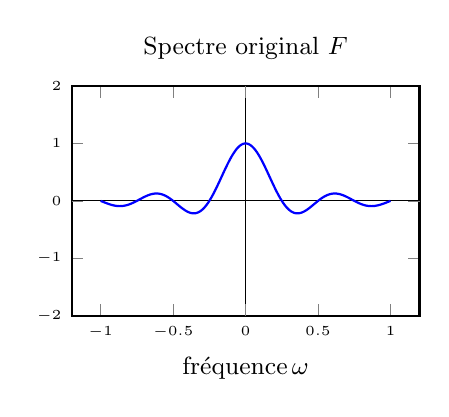
\begin{tikzpicture}
    \begin{axis}[
        title={Spectre original $F$},
        title style={font=\small},
        axis lines=box,
        style=thick,
        xlabel=\(\textnormal{fréquence}\, \omega\),
        xtick={-1, -0.5, 0.5, 1},
        ytick={-2, -1, 1, 2},
        extra x ticks=0,
        extra y ticks=0,
        extra x tick style={grid=major, grid style={black}},
        extra y tick style={grid=major, grid style={black}},
        tick label style={font=\tiny},
        label style={font=\small},
        ymin=-2, 
        ymax=2,
        ]
    \addplot[
        color=blue,
        domain=-1:1,
        samples=200
        ]
    {sin(360*x*2)/ (2*pi*x*2)};
    \end{axis}
    \end{tikzpicture}
    %\hskip 6pt
    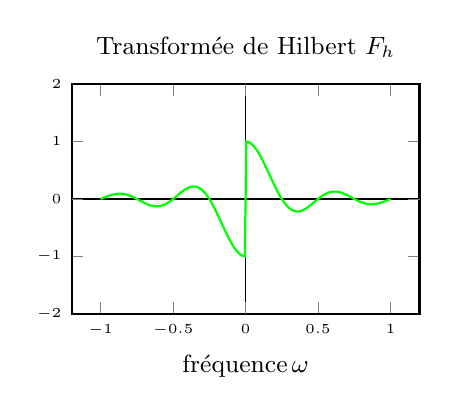
\begin{tikzpicture}
    \begin{axis}[
        title={Transformée de Hilbert $F_h$},
        title style={font=\small},
        axis lines=box,
        style=thick,
        xlabel=\(\textnormal{fréquence}\, \omega\),
        xtick={-1, -0.5, 0.5, 1},
        ytick={-2, -1, 1, 2},
        extra x ticks=0,
        extra y ticks=0,
        extra x tick style={grid=major, grid style={black}},
        extra y tick style={grid=major, grid style={black}},
        tick label style={font=\tiny},
        label style={font=\small},
        ymin=-2, 
        ymax=2,
        ]
    \addplot[
        color=green,
        domain=-1:1,
        samples=200
        ]
    {sign(x)*sin(360*x*2)/ (2*pi*x*2)};
    \end{axis}
    \end{tikzpicture}
    %\hskip 6pt
    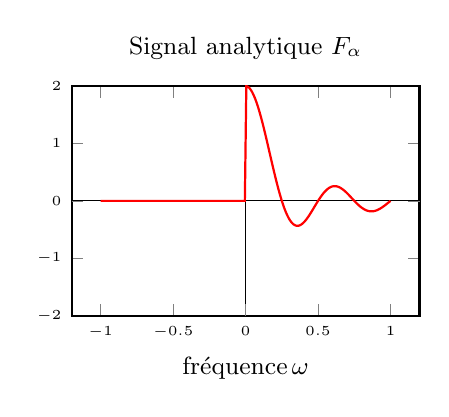
\begin{tikzpicture}
    \begin{axis}[
        title={Signal analytique $F_{\alpha}$},
        title style={font=\small},
        axis lines=box,
        style=thick,
        xlabel=\(\textnormal{fréquence}\, \omega\),
        xtick={-1, -0.5, 0.5, 1},
        ytick={-2, -1, 1, 2},
        extra x ticks=0,
        extra y ticks=0,
        extra x tick style={grid=major, grid style={black}},
        extra y tick style={grid=major, grid style={black}},
        tick label style={font=\tiny},
        label style={font=\small},
        ymin=-2, 
        ymax=2,
        ]
    \addplot[
        color=red,
        domain=-1:1,
        samples=200
        ]
    {(1+sign(x))*sin(360*x*2)/ (2*pi*x*2)};
    \end{axis}
    \end{tikzpicture}

    \caption[Signal analytique pour un signal simple]{Création du signal analytique dans le domaine fréquentiel (seule la partie réelle est montrée). Le signal original réel (gauche), qui présente une symétrie hermitienne, est ajouté à sa transformée de Hilbert (milieu), lui impair, pour former le signal analytique (droite), dépourvu de fréquence négative.}
    \label{fig:complex-analytic-representation}
\end{figure}

En effet, on peut voir le fait de supprimer les composantes de fréquences négatives comme le l'ajout d'un signal impair soigneusement choisi au signal de base.

\begin{equation} \label{eq:2.1}
    F_{\alpha}(\omega) = F(\omega) + F_h(\omega),
\end{equation}

où $F_h(\omega)$ est la « version impaire » du signal $F(\omega)$ :

\begin{equation}
    F_h(\omega) = \left\{
    \begin{array}{ll}
        F(\omega), & \omega > 0 \\
        -F(\omega), & \omega < 0 \\
        0, & \omega = 0,
    \end{array}
    \right.
\end{equation}

que l'on peut reformuler à l'aide de la fonction signe :

\begin{equation}
    F_h(\omega) = \sgn(\omega)\cdot F(\omega).
    \label{eq:2.5}
\end{equation}

On rappelle l'expression de la fonction signe :

\begin{equation}
    \sgn(x) = \left\{
    \begin{array}{ll}
        1, & x > 0 \\
        -1, & x < 0 \\
        0, & x = 0.
    \end{array}
    \right.
\end{equation}

On obtient alors la ré-écriture de l'équation~\ref{eq:2.1} :

\begin{equation}
    F_{\alpha}(\omega) = (1+\sgn(\omega))F(\omega)
\end{equation}

\begin{figure}[h]
    %\noindent
    %\hspace{-10pt}
    \centering
    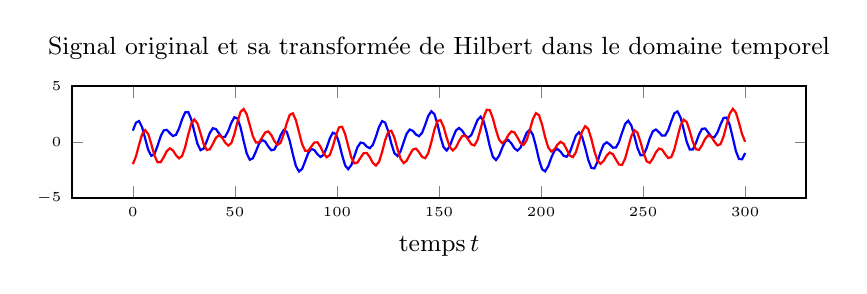
\begin{tikzpicture}
    \begin{axis}[
        title={Signal original et sa transformée de Hilbert dans le domaine temporel},
        title style={font=\small},
        axis lines=box,
        width=0.9\textwidth,
        height=3cm,
        style=thick,
        xlabel=\(\textnormal{temps}\, t\),
        xtick={0, 50, 100, 150, 200, 250, 300},
        ytick={-5, 0, 5},
        tick label style={font=\tiny},
        label style={font=\small},
        ymin=-5, 
        ymax=5,
        ]
    \addplot[
        color=blue,
        domain=0:300,
        samples=200
        ]
    {sin(3*x)+cos(15*x)+sin(30*x)};
    \addplot[
        color=red,
        domain=0:300,
        samples=200
        ]
    {-cos(3*x)+sin(15*x)-cos(30*x)};
    \end{axis}
    \end{tikzpicture}

    \caption[Signal analytique pour un signal complexe]{Exemple de représentation analytique. Le signal original réel (en bleu), et sa transformée de Hilbert imaginaire pure (en rouge).}
    \label{fig:analytic-representation}
\end{figure}


Le signal $F_{\alpha}$ créé est donc dans le domaine fréquentiel de $F$, signal original pair, de représentation purement réelle dans le domaine temporel, et de $F_h$, signal impair, de représentation purement imaginaire dans le domaine temporel, que l'on nomme $f_h$. Dans le domaine temporel, $f_{\alpha}$ est donc un signal complexe, sans composantes de fréquences négatives, c'est un signal analytique, que l'on appelle la \textit{représentation analytique} de $f$ :

\begin{equation}
    f_{\alpha}(t) = \underbrace{f(t)}_\text{réel pur} + \underbrace{f_h(t)}_\text{imaginaire pur}.
\end{equation}

Le signal ajouté pour annuler les fréquences $F_h$ est par ailleurs un objet connu : c'est la \textit{transformée de Hilbert} de $F$. Sa représentation, bien que très simple dans le domaine fréquentiel, est difficile à obtenir et manipuler dans le domaine temporel :

\begin{equation}
    f_h(t) = i \cdot \textnormal{p.v.} \int_{-\infty}^{\infty} \frac{f(t)}{\pi(t-\tau)} \,d\tau,
\end{equation}

où p.v. est la valeur principale de Cauchy, nécessaire pour cette intégrale, qui représente la convolution avec la distribution $\frac 1{\pi t}$ et qui est impropre à cause de la singularité en $t=\tau$. Cependant, dû à la complexité de cet objet, nous utiliserons majoritairement l'expression fréquentielle de la transformée de Hilbert :

\begin{align*}
    &\hil(F) = F_h = \sgn\cdot F \\
    &\mathcal{H}(F) = F_h = \sgn\cdot F
\end{align*}


\subsubsection{Amplitude et phase locales}

Pour comprendre l'intérêt du signal analytique, on étudie d'abord l'exemple d'une fonction sinusoïdale, d'amplitude $A$ et de fréquence $\omega_0$ fixées :

\begin{equation}
    f(t) = A\sin(\omega_0t).
\end{equation}

En utilisant les relations montrées précédemment, on trouve la transformée de Hilbert de $f$ et on calcule sa représentation analytique :

\begin{align}
    f_h(t) &= iA\cos(\omega_0t) \\
    f_{\alpha}(t) &= f(t) + f_h(t) \\
    &= A\sin(\omega_0t)+iA\cos(\omega_0t) \\
    &= Ae^{i\omega_0t}.
\end{align}

Pour une sinusoïde, la transformée de Hilbert est un simple \textit{déphasage} de $-\frac{\pi}2$ du signal original. Or la théorie de Fourier nous indique que n'importe quel signal générique peut être décomposé comme une somme de sinusoïdes. Ainsi la transformée de Hilbert agit de la même manière sur tous les signaux : c'est un déphasage de $-\frac{\pi}2$ de chaque composante fréquentielle qui compose le signal. Le signal $f$ et sa transformée de Hilbert $f_h$ sont dit en \textit{quadrature de phase}, et le signal analytique s'exprime comme une exponentielle complexe.

\bigskip

En fait, puisque tout signal est maintenant représenté comme la somme d'un réel et d'un imaginaire pur, on peut toujours l'exprimer en coordonnées polaires comme une exponentielle complexe, d'amplitude et phase variant au cours du temps :

\begin{equation}
    f_{\alpha} (t) = A(t)e^{i\phi(t)}.
\end{equation}

avec 

\begin{align}
    A(t) &= \sqrt{f(t)^2 + h_h(t)^2} \\
    \phi(t) &= \arctan\left(\frac{f_h(t)}{f(t)}\right).
\end{align}

Cette représentation introduit le concept d'\textit{amplitude locale} et de \textit{phase locale} (ici \textit{temporellement} locales), qui sont deux outils d'analyse particulièrement intéressants pour l'étude approfondie du signal original. L'amplitude locale agit comme une mesure de l'\textit{enveloppe} du signal, et la phase locale comme une mesure de la \textit{forme} du signal. Par exemple, une phase de $0$ indique un extremum, et une phase de $\pm\pi$ indique un passage par zéro. La figure~\ref{fig:local-pha-amp} montre un signal avec son amplitude locale et sa phase locale. À partir uniquement de notre signal initial, on a ainsi créé un outil nous permettant d'obtenir de l'information bien plus intéressante sur l'apparence et les propriétés du signal.

\begin{figure}[h]

    \centering
    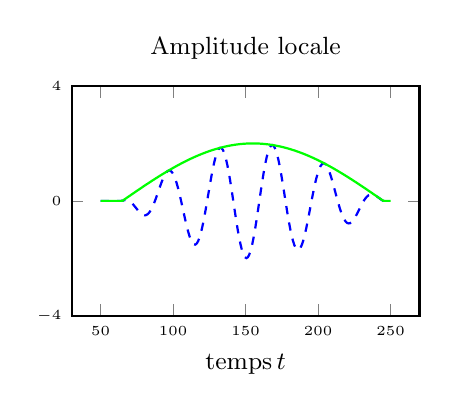
\begin{tikzpicture}
    \begin{axis}[
        title={Amplitude locale},
        title style={font=\small},
        axis lines=box,
        %width=0.9\textwidth,
        %height=3cm,
        style=thick,
        xlabel=\(\textnormal{temps}\, t\),
        xtick={50, 100, 150, 200, 250},
        ytick={-4, 0, 4},
        tick label style={font=\tiny},
        label style={font=\small},
        ymin=-4, 
        ymax=4,
        ]
    \addplot[
        color=blue,
        domain=50:250,
        samples=200,
        style=dashed,
        ]
    {(sign(x-65)-sign(x-245))*sin(10*x+25)*cos(x+25)};
    \addplot[
        color=green,
        domain=50:250,
        samples=200
        ]
    {(sign(x-65)-sign(x-245))*sqrt((0.5*(sin(11*x-40) + sin(9*x-90)))^2 + (sin(10*x+25)*cos(x+25))^2)};
    \end{axis}
    \end{tikzpicture}
    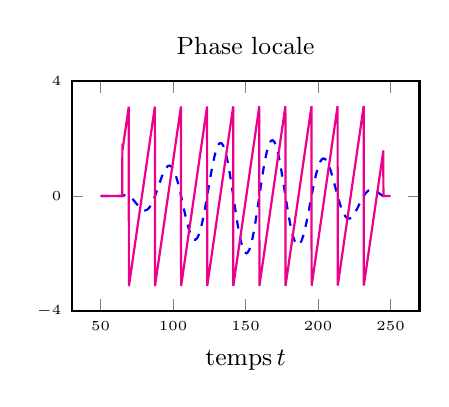
\begin{tikzpicture}
    \begin{axis}[
        title={Phase locale},
        title style={font=\small},
        axis lines=box,
        %width=0.9\textwidth,
        %height=3cm,
        style=thick,
        xlabel=\(\textnormal{temps}\, t\),
        xtick={50, 100, 150, 200, 250},
        ytick={-4, 0, 4},
        tick label style={font=\tiny},
        label style={font=\small},
        ymin=-4, 
        ymax=4,
        ]
    \addplot[
        color=blue,
        domain=50:250,
        samples=200,
        style=dashed,
        ]
    {(sign(x-65)-sign(x-245))*sin(10*x+25)*cos(x+25)};
    \addplot[
        color=magenta,
        domain=50:250,
        samples=2000
        ]
    {(sign(x-65)-sign(x-245))*rad(atan((0.5*(sin(11*x-40) + sin(9*x-90))) / (sin(10*x+25)*cos(x+25))))};
    \end{axis}
    \end{tikzpicture}

    \caption[Informations locales pour un signal simple]{Extraction d'informations locales pour un cosinus modulé par un sinus. L'amplitude locale (gauche) donne l'enveloppe de la sinusoïde, et la phase locale (droite) nous donne de l'information quant à la position dans le cycle d'oscillation.}
    \label{fig:local-pha-amp}

\end{figure}

\subsubsection{Notion d'échelle}
\label{subsubsec:echelle}

L'exemple donné avec la figure~\ref{fig:local-pha-amp} fonctionne bien car le signal est simple, l'interprétation de l'amplitude et la phase locale est claire et visuelle. Pour un signal plus complexe, plus représentatif des signaux que l'on doit souvent étudier, ce n'est pas si facile. La figure~\ref{fig:complex-local-pha-amp} affiche les informations locales du signal de la figure~\ref{fig:analytic-representation}, une somme de trois sinusoïdes de fréquences différentes ; il est moins évident de comprendre ce que les informations locales représentent dans ce cas.

\bigskip

\begin{figure}[h]
    \centering
    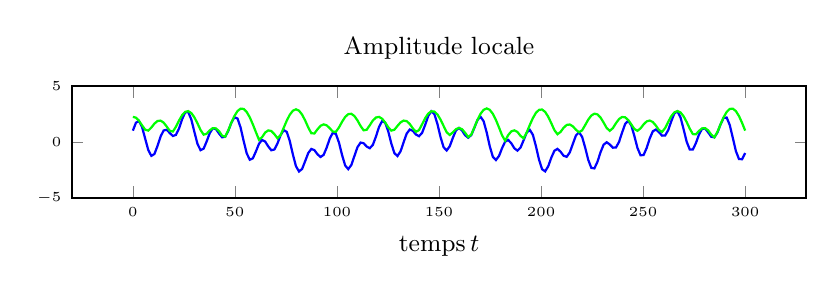
\begin{tikzpicture}
    \begin{axis}[
        title={Amplitude locale},
        title style={font=\small},
        axis lines=box,
        width=0.9\textwidth,
        height=3cm,
        style=thick,
        xlabel=\(\textnormal{temps}\, t\),
        xtick={0, 50, 100, 150, 200, 250, 300},
        ytick={-5, 0, 5},
        tick label style={font=\tiny},
        label style={font=\small},
        ymin=-5, 
        ymax=5,
        ]
    \addplot[
        color=blue,
        domain=0:300,
        samples=200
        ]
    {sin(3*x)+cos(15*x)+sin(30*x)};
    \addplot[
        color=green,
        domain=0:300,
        samples=200
        ]
    {sqrt((sin(3*x)+cos(15*x)+sin(30*x))^2 + (-cos(3*x)+sin(15*x)-cos(30*x))^2)};
    \end{axis}
    \end{tikzpicture}
    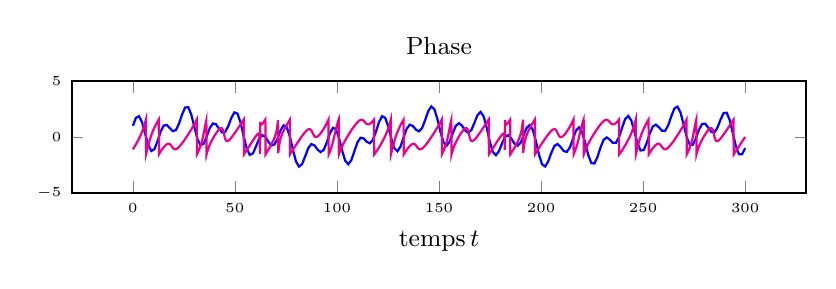
\begin{tikzpicture}
    \begin{axis}[
        title={Phase},
        title style={font=\small},
        axis lines=box,
        width=0.9\textwidth,
        height=3cm,
        style=thick,
        xlabel=\(\textnormal{temps}\, t\),
        xtick={0, 50, 100, 150, 200, 250, 300},
        ytick={-5, 0, 5},
        tick label style={font=\tiny},
        label style={font=\small},
        ymin=-5, 
        ymax=5,
        ]
    \addplot[
        color=blue,
        domain=0:300,
        samples=200
        ]
    {sin(3*x)+cos(15*x)+sin(30*x)};
    \addplot[
        color=magenta,
        domain=0:300,
        samples=3000
        ]
    {rad(atan((-cos(3*x)+sin(15*x)-cos(30*x)) / (sin(3*x)+cos(15*x)+sin(30*x))))};
    \end{axis}
    \end{tikzpicture}    

    \caption[Informations locales pour un signal complexe]{Informations locales pour un signal complexe, somme de plusieurs sinusoïdes. Pour un tel signal, l'interprétation des informations locales est moins évidente.}
    \label{fig:complex-local-pha-amp}
\end{figure}

Le problème à l'analyse de ce signal est le fait qu'il existe plusieurs niveaux de structure, qui interfèrent et rendent l'interprétation des informations locales impossible à l'échelle macroscopique.
Pour extraire de l'information utile, il faut sélectionner et faire l'analyse d'un seul niveau de structure, donc d'échelle.
Pour cela, on filtre les composantes des niveaux qui ne nous intéressent pas.
Pour se faire, il est possible d'utiliser des filtres passe-bande, comme le fait Bridge avec les filtres log-Gabor, un choix commun pour ce genre de pratique.
Un filtre log-Gabor est un filtre défini dans le domaine fréquentiel, qui permet de sélectionner une bande de fréquence centrée autour d'une fréquence centrale $\omega_0$.
Il a une réponse en fréquence de forme gaussienne quand observé en échelle logarithmique :

\begin{equation}
    G(\omega) = \exp\left(-\frac{\log^2(\frac{|\omega|}{\omega_0})}{2\log(\sigma_0)^2}\right).
\end{equation}

Ces filtres sont caractérisés par deux paramètres : la fréquence centrale $\omega_0$, qui contrôle quelle échelle de structure est sélectionnée, et la largeur de bande $\sigma_0$, un paramètre de forme qui contrôle la largeur de la bande de fréquence sélectionnée. Des exemples de filtre log-Gabor sont montrés à la figure~\ref{fig:log-gabor-filters}.

\bigskip

En appliquant un filtre log-Gabor à notre signal avant de lui appliquer la transformée de Hilbert et de déterminer sa représentation analytique, on obtient une représentation locale du signal, centrée autour d'une fréquence $\omega_0$ et d'une échelle $\sigma_0$ que l'on peut faire varier arbitrairement.

\begin{equation}
    F_{\alpha}(\omega) = (1+\sgn(\omega))G(\omega)F(\omega)
\end{equation}

\begin{figure}
    \centering
    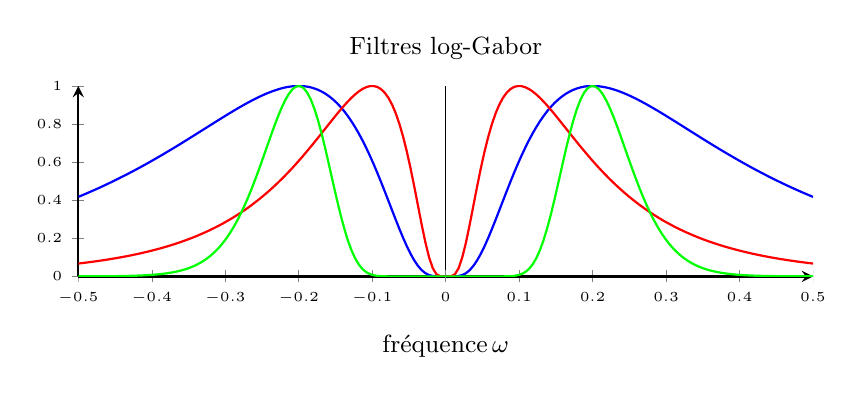
\begin{tikzpicture}
    \begin{axis}[
        title={Filtres log-Gabor},
        title style={font=\small},
        axis lines=left,
        width=0.9\textwidth,
        height=4cm,
        style=thick,
        xlabel=\(\textnormal{fréquence}\, \omega\),
        xtick={-0.5, -0.4, -0.3, -0.2, -0.1, 0.1, 0.2, 0.3, 0.4, 0.5},
        ytick={0, 0.2, 0.4, 0.6, 0.8, 1},
        tick label style={font=\tiny},
        label style={font=\small},
        extra x ticks=0,
        extra x tick style={grid=major, grid style={black}},
        ymin=0,
        ymax=1,
        ]
    \addplot[
        color=blue,
        domain=-0.5:0.5,
        samples=200
        ]
    {exp(-ln(abs(x)/.2)^2 / (2*ln(.5)^2))};
    \addplot[
        color=red,
        domain=-0.5:0.5,
        samples=200
        ]
    {exp(-ln(abs(x)/.1)^2 / (2*ln(.5)^2))};
    \addplot[
        color=green,
        domain=-0.5:0.5,
        samples=200
        ]
    {exp(-ln(abs(x)/.2)^2 / (2*ln(.8)^2))};
    \end{axis}
    \end{tikzpicture}

    \caption[Filtres log-Gabor]{Représentation dans le domaine fréquentiel de filtres log-Gabor de différents paramètres. En rouge, $\omega_0=0.1, \sigma_0 = 0.5$. En bleu, $\omega_0=0.2, \sigma_0 = 0.5$. En vert, $\omega_0=0.2, \sigma_0 = 0.8$.}
    \label{fig:log-gabor-filters}
\end{figure}

En étudiant la réponse du signal sur une large gamme de fréquences et d'échelles, on obtient une représentation locale du signal à différentes échelles, et ainsi extraire de l'information sur les différentes structures du signal. On peut rassembler toutes ces informations dans un graphique appelé scalogramme, qui représente le comportement de la phase locale en fonction du temps et de l'échelle, comme montré à la figure~\ref{fig:scalogram}. On y voit facilement les différents niveaux de structure du signal, et l'interprétation des informations locales devient plus utile car on peut choisir à quel niveau on regarde.

\bigskip

Si l'on compare le modèle du signal analytique à celui de la transformée de Fourier, on remarque que les informations que l'on obtient avec les deux diffèrent et se complètent. La transformée de Fourier nous donne de l'information globale sur tout le signal, mais localisée en termes de fréquence. La représentation analytique, elle, nous donne une information spatialement locale sur le signal, mais sur une bande de fréquences, sélectionnées par un filtre passe-bande. Le modèle d'information locale est donc un compromis entre la localisation spatiale et fréquentielle, et permet d'obtenir une information différente sur le signal.


\begin{figure}
    \centering
    \includegraphics[width=\textwidth]{contenu/resources/images/scalogram}
    \caption[Scalogramme de la phase locale]{Scalogramme de la phase locale pour un signal complexe. La phase locale est représentée en échelle de gris, et varie en fonction du temps (en abscisse) et de l'échelle en nombre de pixels (en ordonnée). Diagramme par Bridge~\cite{bridge_introduction_2018}.}
    \label{fig:scalogram}
\end{figure}


\subsection{Deux dimensions, signal monogène}

Le modèle du signal analytique est utile à l'extraction d'informations locales pour des signaux 1D, et il serait intéressant d'avoir accès à ces informations pour des images, donc des signaux 2D. En effet l'importance de la phase dans l'analyse d'image a déjà été soulignée depuis longtemps~\cite{oppenheim_importance_1981}. Cependant, l'application n'est pas directe dans le cas de deux (ou plus) dimensions, car il y a une notion de direction à considérer. C'est ce que le modèle du signal monogène, proposé par Felsberg et Sommer~\cite{felsberg_monogenic_2001}, permet de faire, et que nous allons développer dans cette partie.

\subsubsection{Construction du signal monogène}

Pour créer la représentation analytique d'un signal 1D, on SY génère un imaginaire pur, en quadrature de phase avec le signal original, en utilisant la transformée de Hilbert. Pour un signal 2D, on a besoin de former deux « parties imaginaires », une pour chaque direction. On ne peut donc pas représenter le signal monogène comme un complexe. Pour un traitement exact, il faudrait utiliser les quaternions, que l'on peut voir comme une extension des nombres complexes à une plus haute dimension. Pour simplifier la compréhension et manipulation, on peut cependant se passer de la théorie des quaternions, et traiter le signal monogène comme s'il avait trois parties réelles distinctes dans un premier temps.
Pour générer les parties impaires du signal, on utilise une généralisation de la transformée de Hilbert à plusieurs dimensions, la \textit{transformée de Riesz}. Soit $f$ un signal d'un espace 2D de la variable $\mathbf{x} = (x, y)^T$, et $F$ sa représentation dans le domaine fréquentiel obtenue par transformée de Fourier 2D, avec $\mathbf{\omega}=(\omega_x, \omega_y)^T$ une fréquence 2D. Alors les parties impaires de $f$, $F_{o1}$ et $F_{o2}$, sont données par :

\begin{align}
    F_{o1}(\mathbf{\omega}) &= \widehat{\mathcal{R}_1(f)}(\mathbf{\omega}) =
        \left\{
        \begin{array}{ll}
            -i\frac{\omega_x}{||\omega||}F(\omega), & \omega > 0 \\
            0, & \omega = 0,
        \end{array}
        \right. \\
    F_{o2}(\mathbf{\omega}) &= \widehat{\mathcal{R}_2(f)}(\mathbf{\omega}) =
        \left\{
        \begin{array}{ll}
            -i\frac{\omega_y}{||\omega||}F(\omega), & \omega > 0 \\
            0, & \omega = 0.
        \end{array}
        \right.
    \label{eq:2.20}
\end{align}

Avec cette définition de $F_{o1}$ et $F_{o2}$, on a que les signaux correspondant dans le domaine spatial sont des signaux à valeurs réelles. En effet un signal 2D à valeurs réelles $f$ a un spectre dont la partie réelle est paire, et la partie imaginaire impaire, soit :

\begin{equation}
    Re\{F(\omega)\} = Re\{F(-\omega)\}, \quad Im\{F(\omega)\} = -Im\{F(-\omega)\}.
\end{equation}

Dans la définition~\ref{eq:2.20}, comme $F$ est le spectre d'un signal réel, on a que $F_{o1}$ et $F_{o2}$ vérifient ces propriétés de symétrie, et donc que les signaux correspondants dans le domaine spatial sont bien réels.

\bigskip

Si l'on compare à comment la transformée de Hilbert est formée~\ref{eq:2.5}, on remarque que ces parties impaires sont des versions généralisées de la transformée de Hilbert, où l'on prend en compte la direction de la fréquence. Chaque composante fréquentielle dans ces parties impaires est déphasée de $-\pi/2$ et mise à l'échelle de telle sorte que l'amplitude soit partagée entre les deux parties.

\bigskip

\begin{figure}
    \centering
    \begin{subfigure}[b]{.3\textwidth}
        \includegraphics[width=\textwidth]{contenu/resources/images/disk}
        \caption{Signal original}
    \end{subfigure}
    \hfill
    \begin{subfigure}[b]{.3\textwidth}
        \includegraphics[width=\textwidth]{contenu/resources/images/r2_disk}
        \caption{Première partie impaire}
    \end{subfigure}
    \hfill
    \begin{subfigure}[b]{.3\textwidth}
        \includegraphics[width=\textwidth]{contenu/resources/images/r1_disk}
        \caption{Seconde partie impaire}
    \end{subfigure}
    \caption[Visualisation du signal monogène pour un disque]{Visualisation du signal monogène pour un disque : le signal original $f$ (gauche), et ses parties impaires $f_{o1}$ (milieu) et  $f_{o2}$ (droite), affichées avec une échelle de couleurs encodant la valeur, de -1 (noir) à +1 (blanc).}
    \label{fig:monogenic-signal-disk}
\end{figure}

On obtient ainsi une expression du signal monogène comme un vecteur à trois composantes, une paire et deux impaires :

\begin{equation}
    f_m(\mathbf{x}) =
    \left[
        \begin{array}{c}
        f_e(\mathbf{x}) \\
        f_{o1}(\mathbf{x}) \\
        f_{o2}(\mathbf{x})
        \end{array}
    \right],
\end{equation}

où $f_e$ est le signal original, indexé par un $e$ pour souligner qu'il représente la partie paire du signal monogène. Une représentation d'un signal et de ses parties impaires est présentée à la figure~\ref{fig:monogenic-signal-disk}. On remarque notamment que les parties impaires détectent des changements verticaux et horizontaux dans le signal. Ceci est dû au fait que la transformée de Riesz présente une ressemblance et une connexion au gradient (l'équation~\ref{eq:2.20} rappelle fortement la définition du gradient, à un facteur près), que présente aussi d'ailleurs la transformée de Hilbert en une dimension. Ce rapport au gradient ne sera cependant pas exploré plus en profondeur dans la suite de ce travail.

\bigskip

Il est aussi commun de se représenter le signal monogène comme un vecteur de deux composantes seulement, une paire et une impaire, où cette dernière est en fait une combinaison des deux parties impaires présentées ici. Cette représentation est plus compacte, mais ce au détriment de la perte d'information sur l'orientation. Elle sera parfois utilisée dans la suite de ce travail :

\begin{equation}
    f_o(\mathbf{x}) = \sqrt{f_{o1}(\mathbf{x})^2 + f_{o2}(\mathbf{x})^2}.
\end{equation}

La transformée de Riesz peut s'exprimer directement dans le domaine spatial, mais comme la transformée de Hilbert, elle n'est représentable que par un objet mathématique compliqué, une intégrale singulière :

\begin{equation}
    R_if(x) = c_d \lim_{\epsilon \to 0}\int_{\mathbb{R}^d\setminus B_\epsilon(x)}\frac{(x_i-t_i)f(t)}{|x-t|^{d+1}}\,dt,
    \label{eq:riesz-transform-spatial}
\end{equation}

pour $i\in\llbracket 0, d\rrbracket$ avec $d$ la dimension, et où $c_d$ est une constante de normalisation dimensionnelle :

\begin{equation}
    c_d = \frac1{\pi\omega_{d-1}} = \frac{\Gamma((d+1)/2)}{\pi^{(d+1)/2}},
\end{equation}

avec $\omega_{d-1}$ le volume de la $(d-1)$-sphère unité. Au vue de la complexité de calcul et de manipulation de cette expression, nous utiliserons plutôt la formulation fréquentielle dans la suite du travail.

\subsubsection{Amplitude, phase et orientation locales}

Avec cet outil qu'est le signal monogène, on peut maintenant étendre les concepts d'informations locales à nos images, qui sont des signaux 2D. En 1D, on a deux parties pour le signal analytique, que l'on représente en coordonnées polaires avec l'amplitude et la phase. En 2D, on a trois coordonnées, que l'on représente donc en coordonnées sphériques où sont définis le rayon, l'angle d'élévation et l'azimut, comme montré en figure~\ref{fig:spherical-representation}.

\bigskip

\begin{figure}
    \centering
    \includegraphics[width=.45\textwidth]{contenu/resources/images/spherical_representation}
    \caption[Représentation du signal monogène en coordonnées sphériques]{Représentation du signal monogène $f_m$ (rouge) en coordonnées sphériques, où les axes sont les différentes parties du signal. Le rayon représente l'amplitude locale, l'angle d'élévation $\phi$ la phase locale, et l'azimut $\theta$ l'orientation locale.}
    \label{fig:spherical-representation}
\end{figure}

L'amplitude locale $A$ représente, comme en 1D, le rayon de la représentation :

\begin{align}
    A(\mathbf{x}) &= \sqrt{f_e(\mathbf{x})^2 + f_{o1}(\mathbf{x})^2 + f_{o2}(\mathbf{x})^2} \\
    &= \sqrt{f_e(\mathbf{x})^2 + f_o(\mathbf{x})^2}.
\end{align}

La phase locale $\phi$ mesure l'angle entre la partie paire $f_e$ et la partie impaire combinée $f_o$, et représente donc l'angle d'élévation de la représentation :

\begin{equation}
    \phi(\mathbf{x}) = \arctan\left(\frac{f_o(\mathbf{x})}{f_e(\mathbf{x})}\right).
\end{equation}

Enfin l'orientation locale $\theta$ complète la représentation en donnant l'angle d'azimut, soit la direction dominante dans l'image à cet endroit, exprimé comme l'orientation de la partie impaire $f_o$ :

\begin{equation}
    \theta(\mathbf{x}) = \arctan\left(\frac{f_{o2}(\mathbf{x})}{f_{o1}(\mathbf{x})}\right).
\end{equation}

La figure~\ref{fig:monogenic-local-representation} montre un exemple de représentation locale pour une image, avec l'amplitude, la phase et l'orientation locales.

\bigskip

\begin{figure}
    \centering
    \includegraphics[width=\textwidth]{contenu/resources/images/local_information_monogenic}
    \caption[Représentation locale du signal monogène]{Représentation locale du signal monogène pour une image, avec l'amplitude (gauche), la phase (milieu) et l'orientation (droite) locales. Image par Bridge~\cite{bridge_introduction_2018}.}
    \label{fig:monogenic-local-representation}
\end{figure}

Le changement de représentation est réversible, et on peut retrouver le signal monogène à partir des informations locales :

\begin{equation}
    f_m(\mathbf{x}) = A(\mathbf{x})\left[
        \begin{array}{c}
        \cos(\phi(\mathbf{x})) \\
        \sin(\phi(\mathbf{x}))\cos(\theta(\mathbf{x})) \\
        \sin(\phi(\mathbf{x}))\sin(\theta(\mathbf{x}))
        \end{array}
    \right].
\end{equation}

L'image originale notamment s'exprime simplement par $f(\mathbf{x}) = A(\mathbf{x})\cos(\phi(\mathbf{x}))$. Nous utiliserons cette formule plus tard dans nos travaux pour reconstruire nos images après avoir modifié leurs informations locales.

\bigskip

Comme pour le signal analytique en 1D, il est intéressant d'utiliser des filtres pour sélectionner un niveau d'échelle à analyser, afin d'extraire de l'information sur certains niveaux de structure en particulier. Ici encore, on peut utiliser des filtres log-Gabor pour séléctionner les parties du signal qui nous intéressent.

\bigskip

\begin{figure}
    \centering
    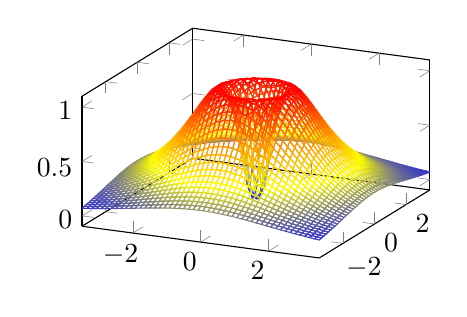
\begin{tikzpicture}
    \begin{axis}[
        colormap/hot,
%        xtick={-.5, 0, .5},
%        ytick={-.5, 0, .5},
%        ztick={-1, 0, 1}
    ]
        \addplot3[
        mesh,
        samples=50,
        domain=-3.5:3.5,
        ]
        {exp(-(ln(sqrt(x^2+y^2))^2)/(2*ln(.5)^2))};
    \end{axis}
    \end{tikzpicture}

    \caption[Filtre log-Gabor en 2D]{Représentation en domaine fréquentiel d'un filtre log-Gabor. Comme en 1D, le filtre sélectionne une bande de fréquence centrée autour d'une fréquence centrale $\omega_0$, et de largeur de bande $\sigma_0$.}
    \label{fig:2D-log-gabor}
\end{figure}

Avec ces filtres, on calcule les parties paires et impaires du signal en sélectionnant plusieurs échelles différentes, et on obtient ainsi une représentation locale qui met en valeur différents niveaux de structure présents dans l'image. La figure~\ref{fig:cameraman-monogenic} montre une image et son signal monogénique, calculé sur plusieurs niveaux d'échelle.

\begin{figure}
    \centering
    \includegraphics[width=.75\textwidth]{resources/images/cameraman_monogenic}
    \caption[Signal monogène calculé pour plusieurs niveaux d'échelle]{Image originale (gauche) et son signal monogène (droite), calculé sur plusieurs niveaux d'échelle. Dans l'image de droite : en colonne les différentes parties, paire $f_e$ (gauche), impaire 1 $f_{o1}$ (milieu) et impaire 2 $f_{o2}$ (droite). En ligne les longueurs d'onde centrale $\lambda_0 = 2\pi/\omega_0$, caractéristiques de l'échelle de structure détectée : $\lambda_0 = 20$~pixels (haut), $\lambda_0 = 60$~pixels (milieu), $\lambda_0 = 100$~pixels (bas). Pour référence, la taille de l'image originale est 256 $\times$ 256 pixels. Image par Bridge~\cite{bridge_introduction_2018}.}
    \label{fig:cameraman-monogenic}
\end{figure}



\bigskip
{\color{red} SY cadre de travail}
Maintenant que notre cadre de travail pour le restant du manuscript, le signal monogène, a été plus formellement introduit, nous allons pouvoir nous intéresser RE au cadre que nous avons choisi pour travailler à différents niveaux de structure. Bridge présente dans son article~\cite{bridge_introduction_2018} un cadre de travail utilisant les filtres log-Gabor, qui possèdent une expression complexe dans le domaine temporel. Pour nos travaux, nous avons utilisé une autre méthode de représentation, la pyramide de Riesz, plus simple à calculer et manipuler, et qui nous permet de nous concentrer sur l'analyse de textures. Nous allons maintenant présenter cette pyramide de Riesz, et montrer comment elle peut être utilisée pour l'analyse de textures.

\section{Pyramide de Riesz}

% Pyramide d'images inventée par Burt et Adelson~\cite{burt_laplacian_1983} pour la compression d'images.
L'idée d'utiliser une pyramide d'images est introduite par Simoncelli et al.~\cite{simoncelli_shiftable_1992}, {\color{red}REFOLMURER dans le but d'avoir une représentation possédant des bonnes propriétés d'études.}. C'est une méthode de représentation multi-échelle d'une image.
% AVANTAGES de la pyramide d'images de Simoncelli, la complex steerable pyramid :
% - steerable, invariance par rotation
% - invariance par translation et mise à l'échelle
% - avoids spatial aliasing
SY Conceptuellement, une pyramide d'images remplit la même fonction qu'une banque de filtres, comme les filtres log-Gabor utlisés par Bridge : on décompose une image en s'intéressant successivement à différentes bandes de fréquences, afin d'extraire de l'information localisée en fréquence. La pyramide que nous utilisons, inspirée de Wadhwa et al.~\cite{wadhwa_phase_based_2013}, est construite en formant dans un premier temps la pyramide de Gauss, puis de Laplace de l'image, qui elle nous sert à avoir une méthode de reconstruction de notre image. On applique ensuite la transformée de Riesz à tous les étages de la pyramide, pour obtenir le signal monogène de chaque niveau. De là, on extrait les informations locales à tous les niveaux de structure, informations qui seront ultérieurement utilisées pour l'analyse et la synthèse de nos textures.

\subsection{Pyramide gaussienne}

RE La méthode de pyramide d'images est une méthode de représentation multi-échelle d'une image, répandue dans les domaines de la vision par ordinateur et du traitement d'images. Initialement introduite par Burt et Adelson~\cite{burt_laplacian_1983} pour la compression d'images, elle permet d'étudier une image à différents niveaux de résolution, afin de faciliter la détection de motifs en sélectionnant le niveau d'échelle correspondant au motif recherché. Elle est ensuite étendue par Simoncelli et al.~\cite{simoncelli_shiftable_1992} pour RE avoir une représentation possédant des bonnes propriétés d'études.

\bigskip

Il existe deux types principaux de pyramide, passe-bas et passe-bande. Pour créer une pyramide passe-bas, aussi dite de Gauss, on procède itérativement suivant les deux étapes qui suivent :

\bigskip

\begin{itemize}
    \item une étape de \textit{lissage} (ou filtrage) de l'image, qui consiste à appliquer un filtre passe-bas à l'image, afin de supprimer les hautes fréquences. On obtient ainsi une image lissée, où les détails fins ont été supprimés ;
    \item une étape de \textit{sous-échantillonnage}, qui consiste à réduire la taille de l'image en gardant un pixel sur deux dans chaque direction. On obtient ainsi une image de moitié de la taille de l'image originale.
\end{itemize}

On répète ces deux étapes sur l'étage nouvellement créé, et ce jusqu'à atteindre la profondeur désirée. On se retrouve ainsi avec une collection d'images de plus en plus petites et de moins en moins raffinées (en termes de résolution), qui peut graphiquement être représentée comme une pyramide, en superposant les étages du plus grand au plus petit, comme montré à la figure~\ref{fig:gaussian-pyramid}.

\begin{figure}[h]
    \centering

    \begin{subfigure}{.3\textwidth}
        \centering
        \includegraphics[width=\textwidth]{contenu/resources/images/gauss_0}
        \caption{Image originale}
    \end{subfigure}
    \hfill
    \begin{subfigure}{.3\textwidth}
        \centering
        \includegraphics[width=\textwidth]{contenu/resources/images/gauss_3}
        \caption{Étage 3}
    \end{subfigure}
    \hfill
    \begin{subfigure}{.3\textwidth}
        \centering
        \includegraphics[width=\textwidth]{contenu/resources/images/gauss_5}
        \caption{Étage 5}
    \end{subfigure}
%    \hfill
%    \begin{subfigure}{.22\textwidth}
%        \centering
%        \includegraphics[width=\textwidth]{contenu/resources/images/gauss_3}
%        \caption{Étage 3}
%    \end{subfigure}

    \caption[Pyramide de Gauss]{Pyramide de Gauss. De gauche à droite, on descend dans les étages de plus en plus petits.}
    \label{fig:gaussian-pyramid}
\end{figure}

Plusieurs noyaux de lissage différents ont été proposés dans la littérature, comme la famille des noyaux binomiaux que nous utilisons dans notre implémentation RE en suivant l'exemple de la bibliothèque de traitement d'images OpenCV. Notre noyau de convolution s'exprime à l'aide des coefficients binomiaux :

\begin{equation}
    k = \frac{1}{256}\left[
        \begin{array}{ccccccc}
            1 & 4 & 6 & 4 & 1 \\
            4 & 16 & 24 & 16 & 4 \\
            6 & 24 & 36 & 24 & 6 \\
            4 & 16 & 24 & 16 & 4 \\
            1 & 4 & 6 & 4 & 1
        \end{array}
    \right],
\end{equation}

Il est intéressant de constater que les pyramides gaussiennes sont notamment utilisées dans la synthèse de texture, où elles permettent de résoudre des problèmes d'échantillonnage. En effet les MIP maps employées pour remédier au sous-échantillonnage sont un pré-calcul des textures à différents niveaux de résolution ; ce sont des pyramides gaussiennes.

\begin{figure}
    \centering
    \includegraphics[width=.25\textwidth]{contenu/resources/images/image_pyramid_placeholder}
    \caption[Représentation pyramidale des étages de la pyramide de Gauss]{Représentation en pyramide des étages de la pyramide de Gauss. {\color{red}PLACEHOLDER CREDIT WIKIPEDIA}}
    \label{fig:pyramid-gauss}
\end{figure}

\subsection{Pyramide laplacienne}

La pyramide laplacienne est une autre forme de pyramide, et correspond à un type passe-bande. Comme l'expliquent Burt et Adelson~\cite{burt_laplacian_1983} RE L'intérêt de la pyramide laplacienne réside dans le fait que dans une image, les pixels voisins sont souvent hautement corrélés. Ainsi encoder une image en termes de valeur de pixels n'est pas le plus efficace, puisqu'on a de la redondance d'information. Pour encoder plus efficacement une image, on a besoin d'une représentation plus compacte, et qui décorelle les pixels voisins. La pyramide laplacienne est une méthode qui répond efficacement à ces deux problématiques.

\subsubsection{Construction de la pyramide}

Plutôt que d'encoder la valeur même de chaque pixel, on prédit la valeur que le pixel devrait avoir, et on encode l'erreur de prédiction. La valeur prédite de chaque pixel est obtenue en calculant une moyenne pondérée locale centrée autour du pixel. On crée donc dans un premier temps une image lissée en convoluant l'image avec un filtre correspondant au calcul de la moyenne pondérée. Cette image encode les corrélations locales de l'image, au niveau d'échelle correspondant au filtre choisi, et représente les éléments redondants que l'on cherche à réduire. Pour se faire, on soustrait cette image à l'originale, et on obtient une image exprimant l'erreur de prédiction pour chaque pixel. On a ainsi la relation :

\begin{equation}
    L = I - k * I,
\end{equation}

avec $I$ l'image originale, $L$ l'image d'erreur de prédiction, et $k$ le filtre de moyenne pondérée. Pour la compression d'images, l'intérêt se trouve dans cette ré-écriture, car les pixels de $L$ sont décorrélés et de faible valeur, donc encodables avec peu de bits, et $k*I$ est une image lissée, qui peut être sous-échantillonnée pour obtenir une image de moitié de taille. On n'encode alors que ces deux images, et on obtient ainsi une représentation plus compacte de l'image originale.

\bigskip

On peut répéter ce processus itérativement, en appliquant à chaque fois le même filtre à l'image lissée de résolution inférieure. On enregistre alors seulement les images d'erreur, dont la taille est divisée par 4 à chaque fois, et la dernière image lissée, de taille $N/2^{2d}$, avec $N$ la taille de l'image initiale et $d$ la profondeur désirée. Encore une fois, on peut se représenter cette collection d'images comme une pyramide, en les superposant de la plus grande à la plus petite.

\bigskip

Le filtre de lissage utilisé est un filtre passe-bas, qui moyenne localement l'image, c'est en fait le même genre que l'on utilise pour créer une pyramide gaussienne. En fait, pour construire une pyramide laplacienne, on utilise souvent la pyramide gaussienne de l'image, qui représente toutes les images lissées. On calcule la pyramide gaussienne, puis ensuite la pyramide laplacienne en soustrayant à chaque étage de la pyramide gaussienne l'étage de plus basse résolution, et on obtient ainsi les images d'erreur de prédiction. En se faisant, on fait une légère approximation des images lissées. En effet dans la pyramide gaussienne, il y a une légère perte d'informations entre les étages, puisque l'on supprime des pixels à chaque fois.

\bigskip

Lorsque l'on veut soustraire une image lissée à son image de taille originale, il faut passer par une étape d'expansion. Une méthode communément utilisée pour l'expansion consiste à doubler la taille de l'image, en insérant des zéros entre chaque pixel, puis à appliquer un filtre passe-bas à l'image résultante. On obtient ainsi une image de taille double, qui est une approximation de l'image lissée. On peut alors soustraire cette image à l'image originale, et on obtient l'image d'erreur de prédiction.

\begin{figure}
    \centering
    \includegraphics[width=.75\textwidth]{contenu/resources/images/gauss_laplace_pyramid}
    \caption[Relation entre pyramide gaussienne et laplacienne]{Processus de création de la pyramide laplacienne à partir de ma pyramide gaussienne. Image par Jebamalar et Sutha~\cite{jebamalar_design_2014}.}
    \label{fig:gauss-laplace-pyramid}
\end{figure}

\subsubsection{Reconstruction de l'image}

Une fois une image décomposée en pyramide laplacienne, on peut la stocker en enregistrant les images d'erreur de prédiction et l'image lissée de plus basse résolution. Pour reconstruire l'image originale, on procède itérativement. On additionne le résidu basse fréquences, l'image la plus lissée de la pyramide, à la dernière image d'erreur, pour former une image moins lissée. On répète alors le processus, en additionnant à chaque fois l'image lissée obtenue à l'image d'erreur suivante, jusqu'à obtenir l'image originale.

\bigskip

Lorsque l'on utilise une pyramide gaussienne pour créer une pyramide laplacienne, il faut cependant faire attention à la taille des images, qui est divisée par 4 à chaque étage. Pour cela, on étend à chaque étape les images lissées, en utlisant la même opération d'expansion que celle utilisée pour la création de la pyramide. On s'assure ainsi d'opérer sur des images de même taille. Comme à la construction, la reconstruction des images lissées comporte une petite approximation. Puisque l'on travaille avec des images de taille différente, on a perdu de l'information entre les étages. Cependant, à cette étape on additionne les reconstructions d'images lissées, celles qui ont précédemment été soustraites pour la construction. Ainsi, les deux s'annulent, et on a une reconstruction parfaite de notre image originale.

\begin{figure}
    \centering
    \includegraphics[width=.85\textwidth]{contenu/resources/images/laplacian_pyramid_reconstruction}
    \caption[Reconstruction d'une image à partir de sa pyramide laplacienne]{Reconstruction d'une image à partir de sa pyramide laplacienne. $f_i$ les images de la pyramide gaussienne, $h_i$ celles de la pyramide laplacienne, et $l_i$ les images lissées étendues. Image de \href{https://web.archive.org/web/20230203082428/http://sepwww.stanford.edu/data/media/public/sep/morgan/texturematch/paper_html/node3.html}{Stanford Exploration Project}.}
    \label{fig:laplace-reconstruction}
\end{figure}

\subsection{Pyramide de Riesz}

La pyramide de Riesz est une extension de la pyramide laplacienne. C'est le cadre qui nous permet d'étudier le signal monogène d'une image à différents niveaux d'échelle. On la construit simplement en appliquant la transformée de Riesz à chaque étage de la pyramide laplacienne. On calcule alors les informations locales de chaque étage, que nous mettons ensuite en relation dans nos travaux afin d'extraire plus d'information de notre image.

\bigskip

\begin{figure}
    \centering
    \includegraphics[width=.65\textwidth]{contenu/resources/images/riesz_pyramid_cameraman}
    \caption[Pyramide de Riesz]{Différents étages de notre pyramide de Riesz, calculée avec la transformée de Riesz approximée. En colonne, les différentes composantes : l'image originale de la pyramide laplacienne (gauche), puis les deux composantes de Riesz (milieu et droite). En ligne, les différents étages de la pyramide : étage 0 (haut), étage 2 (milieu) et étage 3, le dernier (bas).}
    \label{fig:riesz-pyramid-cameraman}
\end{figure}

Pour des raisons de vitesse de calcul et de simplicité d'implémentation, nous n'utilisons cependant pas la vraie transformée de Riesz, qui nécessiterait une transformation de l'image dans le domaine de Fourier, ou le calcul d'une intégrale singulière (voir~\ref{eq:riesz-transform-spatial}). À la place, nous reprenons l'approximation utilisée par Wadhwa et al.~\cite{wadhwa_riesz_2014}, qui se calcule directement dans le domaine spatial en utilisant les filtres à réponse impulsionnelle finie $[-0.5, 0, 0.5]$ et $[-0.5, 0, 0.5]^T$, dont les réponses en fréquence sont :

\begin{equation}
    -i\sin(\omega_x) \quad \text{et} \quad -i\sin(\omega_y).
\end{equation}

Cette approximation donne de bons résultats dans notre pyramide, car les filtres ont une réponse équivalente aux alentours de $\frac\pi2$, où se concentre la majorité de l'énergie de nos images dans la pyramide laplacienne~\cite{wadhwa_riesz_2014}. En $0$, la différence notable entre les filtres n'est pas très grave, puisque le contenu fréquentiel est très faible. On rappelle en effet que la pyramide laplacienne est formée en soustrayant à chaque étage une image lissée qui correspond au contenu basse fréquence. Wadhwa et al. proposent une méthode pour calculer une meilleure approximation de la transformée de Riesz à l'aide de filtres finis de plus haut ordre. Nous n'avons cependant pas implémenté cette méthode, car l'approximation basique nous donne déjà de bons résultats. Pour avoir de meilleurs résultats, nous aurions plutôt cherché à implémenter un calcul de la transformée de Riesz passant par le domaine fréquentiel et utilisant la transformée de Fourier.

{\color{red}VOIR TRAVAUX LÉO}


\bigskip

\begin{figure}
    \centering
    \includegraphics[width=.65\textwidth]{contenu/resources/images/riesz_approximation}
    \caption[Approximation de la transformée de Riesz]{Comparaison de l'application de la transformée de Riesz (gauche) et de son approximation (droite) pour un niveau de pyramide. Les tranches horizontales en jaune sur les images (a) et (b) sont représentés dans le diagramme en (c).}
    \label{fig:riesz-approximation}
\end{figure}

Après avoir fait la transformée de Riesz, on peut calculer pour chaque étage les images d'informations locales, amplitude, phase et orientation.

\bigskip

\begin{figure}[hp]
    \centering
    \includegraphics[width=.90\textwidth]{contenu/resources/images/riesz_pyramid_pasta}
    \caption[Informations locales de la pyramide de Riesz]{Informations locales de la pyramide de Riesz. En colonne, les différentes composantes : en colonne, les différentes informations locales : amplitude (gauche), phase (milieu) et orientation (droite). En ligne les différentes étages de la pyramide, du premier (haut) au dernier (bas).}
    \label{fig:riesz-pyramid-local}
\end{figure}

Avec cette implémentation de la pyramide de Riesz, nous avons défini notre cadre d'étude multi-résolutionnel local. Nous allons voir dans la prochaine partie comment nous l'utilisons afin d'extraire de l'information sur nos textures.

\section{Congruence de phase}

Le modèle de l'énergie locale est un modèle de détection de caractéristiques saillantes dans une image. Introduit par Morrone et al~\cite{morrone_mach_1986, morrone_feature_1987},il explique la présence de points saillants, tels que des bords et des coins, par l'alignement des phases locales de l'image. Il est basé sur l'observation que les bords et les coins sont des structures résultant de la superposition de sinusoïdes en phase les unes avec les autres. Contrairement aux autres méthodes de détection de caractéristiques, comme celles de Sobel ou Canny, ce modèle est insensible aux variations de luminosité et de grossissement. Les méthodes par gradient utilisent en effet un seuillage pour déterminer les bords, qui dépend de la luminosité et du niveau de zoom de l'image. À l'inverse, le modèle de l'énergie locale permet le calcul de la congruence de phase, une grandeur à valeurs dans $[0, 1]$ mesurant uniformément la présence de caractéristiques dans une image et, de façon intéressante, la \textit{proximité} à un élément caractéristique. C'est cette grandeur à laquelle nous nous intéressons dans la partie qui suit.

\bigskip

La formulation initiale de la congruence de phase utilise les coefficients de la série de Fourier du signal. Cependant, cette formulation comporte trois problèmes : elle est difficile à calculer et manipuler, elle ne permet pas une bonne localisation de l'information (le même problème qui nous pousse à utiliser un cadre de travail multi-résolutionnel pour l'étude du signal monogène), et RE elle ne prend pas en compte la répartition des fréquences en phase. La solution à ces problèmes se fait par différents moyens, dans un premier temps en 1D, puis en 2D.

\subsubsection{Énergie locale}

Tout d'abord, Venkatesh et Owens~\cite{venkatesh_energy_1989} montrent qu'il existe une relation directe entre la congruence de phase et l'énergie locale. Ils mettent ainsi en lumière une expression simplifiée de la congruence de phase :

\begin{equation}
    PC(x) = \frac{E(x)}{\sum_{n=0}^{+\infty} D_n},
\end{equation}

avec $E(x) = \sqrt{f^2(x) + f_h^2(x)}$ l'énergie locale et $D_n$ les coefficients d'amplitude de la série de Fourier du signal :

\begin{equation}
    f(x) = \sum_{n=0}^{+\infty} D_n\cos(n\omega x + \phi_n).
    \label{eq:phase-congruence-energy}
\end{equation}


\subsubsection{Contexte multi-résolutionnel}

Pour obtenir de l'information localisée en termes de fréquence, Kovesi des ondelettes, sous forme de banque de filtres passe-bande, pour sélectionner successivement différents niveaux d'échelle. Il utilise pour cela des filtres de Gabor, très similaires à ceux présentés dans la section introduisant le signal monogène~\ref{subsubsec:echelle}. En faisant la convolution du signal par ces filtres, il obtient de l'information localisée à la fois spatialement et fréquentiellement :

\begin{equation}
    A_n(x) = \sqrt{(f(x)*M^e_n)^2 + (f(x)*M^o_n)^2},
    \label{eq:local-scale-amplitude}
\end{equation}

et

\begin{equation}
    \phi_n(x) = \arctan\left(\frac{f(x)*M^o_n}{f(x)*M^e_n}\right),
\end{equation}

avec $M^e_n$ et $M^o_n$ les filtres passe-bande, paire et impaire, au niveau d'échelle $n$. À noter que le $n$ dans l'équation~\ref{eq:local-scale-amplitude}, entre 1 et $N$ (le nombre de nivaux d'échelle considéré), désigne le niveau d'échelle fréquentiel. Ce n'est pas le même que celui dans l'équation de la série de Fourier~\ref{eq:phase-congruence-energy} qui, lui, représente les différentes sinusoïdes qui forment le signal. En regardant le scalogramme représenté à la figure~\ref{fig:phase-congruence-scalogram} qui représente l'analyse du signal par la banque de filtres, on voit l'intérêt de la congruence de phase : les points saillants sont ceux où la phase est alignée à travers tous les niveaux d'échelle.

\bigskip

\begin{figure}
    \centering
    \includegraphics[width=.85\textwidth]{contenu/resources/images/phase_congruence_scalogram}
    \caption[Scalogramme d'un signal présentant des points caractéristiques]{Signal 1D et ses scalogrammes de phase et d'amplitude. L'abscisse des scalogrammes sont les mêmes que celui du signal, et les ordonnées représentent à la fréquence en échelle logarithmique (valeurs croissantes de bas en haut). Les astérisques marquent les transitions abruptes dans le signal, et correspondent aux instants où la phase est alignée à travers tous les niveaux d'échelle ; ce sont des points où la congruence de phase est élevée. Image par Kovesi~\cite{kovesi_image_1995}.}
    \label{fig:phase-congruence-scalogram}
\end{figure}

Avec les composantes filtrées à différents niveaux d'échelle du signal, on obtient une nouvelle expression de la congruence de phase, qui prend en compte la localisation fréquentielle :

\begin{equation}
    PC(x) = \frac{E(x)}{\sum_{n=1}^{N} A_n(x)} = \frac{\sqrt{F^2(x)+F_H^2(x)}}{\epsilon + \sum_{n=1}^{N}},
\end{equation}

avec $F$ et $F_H$ une reconstruction du signal et de sa transformée de Hilbert respectivement, à partir des composantes filtrées :

\begin{align}
    F(x) &= \sum_{n=1}^{N} f(x)*M_n^e, \,\text{et}\\
    F_H(x) &= \sum_{n=1}^{N} f(x)*M{_n^o},
\end{align}

et $\sum_{n=1}^{N} A_n(x)$ la somme des amplitudes locales à tous les niveaux d'échelle :

\begin{equation}
    \sum_{n=1}^{N} A_n(x) = \sum_{n=1}^{N} \sqrt{(f(x)*M^e_n)^2 + (f(x)*M^o_n)^2}
\end{equation}

et $\epsilon$ une petite constante positive qui assure la stabilité numérique de l'expression quand la somme des amplitudes est très petite. Dans notre implémentation, on utilise $\epsilon = 0.01$.

\bigskip

La reconstruction du signal et de sa transformée de Hilbert est possible lorsque l'on choisit avec soin les filtres de la transformée par ondelettes, de telle sorte que leur fonction de transfert se superposent lorsqu'additionnées et recouvrent l'entièreté du spectre du signal, comme montré dans la figure~\ref{fig:wavelet-spectrum-coverage}.

\begin{figure}
           \centering
           \includegraphics[width=.60\textwidth]{contenu/resources/images/wavelet_spectrum_coverage}
           \caption[Choix des ondelettes pour recouvrir le spectre et permettre la reconstruction du signal]{Banque d'ondelettes choisie de sorte à recouvrir une large couverture du spectre. On voit les ondelettes (haut) et leur fonction de transfert (milieu), et la fonction de transfert de la somme des ondelettes (bas). Image par Kovesi~\cite{kovesi_image_1995}.}
           \label{fig:wavelet-spectrum-coverage}
\end{figure}

\subsubsection{Répartition des fréquences}

La congruence de phase mesure l'alignement des phases à différents niveaux de fréquence, il est donc important qu'une large bande de fréquences soit couverte, afin d'avoir un indicateur significatif. Ceci n'est pas le cas lorsque le signal a une réponse en fréquence restreinte, dans le cas d'un signal simple ou lissé par exemple. La congruence de phase prend alors des valeurs trop grandes sur des plages trop larges du signal, comme montré dans la figure~\ref{fig:phase-congruency-spread}.

\bigskip

\begin{figure}
    \centering
    \begin{subfigure}{.22\textwidth}
        \centering
        \includegraphics[width=\textwidth]{contenu/resources/images/disk}
        \caption{Image originale\\}
    \end{subfigure}
%    \hfill
    \begin{subfigure}{.22\textwidth}
        \centering
        \includegraphics[width=\textwidth]{contenu/resources/images/disk_blur}
        \caption{Image lissée}
    \end{subfigure}
    \\
    \begin{subfigure}{.22\textwidth}
        \centering
        \includegraphics[width=\textwidth]{contenu/resources/images/pc_blur_nospread}
        \caption{Congruence de phase sans pondération}
    \end{subfigure}
%    \hfill
    \begin{subfigure}{.22\textwidth}
        \centering
        \includegraphics[width=\textwidth]{contenu/resources/images/pc_blur_spread}
        \caption{Congruence de phase avec pondération}
    \end{subfigure}

    \caption{Comparaison de la congruence de phase pour une image lissée par un noyau gaussien, avec et sans pondération par la répartition de la réponse en fréquence.}
    \label{fig:phase-congruency-spread}
\end{figure}

Pour remédier à ce problème, on construit une fonction de pondération qui diminue l'importance des points où la réponse en fréquence est restreinte. On mesure la répartition de la réponse en fréquence en comparant la plus grande amplitude locale à celles des autres niveaux d'échelle :

\begin{equation}
    s(x) = \frac1N\left(\frac{\sum_{n=1}^{N}A_n(x)}{\epsilon + A_{max}(x)}\right),
\end{equation}

où $A_{max}(x)$ la plus grande amplitude parmi ces niveaux et $\epsilon$ est encore une petite constante positive qui assure la stabilité numérique de l'expression. On otient ainsi une mesure de la répartition de la réponse en fréquence à valeurs entre 0 et 1, qui nous permet de construire notre fonction de pondération avec la fonction sigmoïde :

\begin{equation}
    W(x) = \frac{1}{1 + \exp^{g(c-s(x))}},
\end{equation}

avec $c$ la valeur de coupure en-dessous de laquelle on considère que la réponse en fréquence est restreinte, et $g$ un paramètre de gain qui contrôle la précision de la coupure. Dans la pratique, on choisit les valeurs $c = 0.4$ et $g = 10$, qui donne des résultats satisfaisants.

On obtient ainsi une fonction de pondération qui vaut 1 lorsque la réponse en fréquence est uniformément répartie, et qui décroit lorsque la réponse en fréquence est restreinte. On peut alors ré-écrire la congruence de phase en prenant en compte cette fonction de pondération :

\begin{equation}
    PC(x) = \frac{W(x)E(x)}{\epsilon + \sum_{n=1}^{N} A_n(x)}.
\end{equation}

\subsubsection{Extension à deux dimensions}

Pour étendre la méthode en deux dimensions, Kovesi utilise une banque de filtres de Gabor 2D auxquels il applique une fonction d'étalement gaussienne, perpendiculairement à la direction du filtre. En variant l'orientation des filtres, il s'assure de recouvrir totalement le spectre de l'image. L'expression de la congruence de phase s'étend pour prendre en compte toutes les orientations :

\begin{equation}
    PC(\mathbf{x}) = \frac{\sum_{o\in \mathcal{O}} W_o(x)E_o(\mathbf{x})}{\epsilon + \sum_{o \in \mathcal{O}}\sum_{n=1}^{N} A_{no}(\mathbf{x})}
\end{equation},

où $\mathcal{O}$ est l'ensemble des orientations utilisées dans la banque de filtres. Le calcul de la répartition des fréquences $W_o(x)$ doit aussi se faire pour chaque orientation.

\subsubsection{Utilisation du cadre multi-résolutionnel local de Riesz}

Nous souhaitons appliquer le modèle de la congruence de phase pour synthétiser des textures présentant de la structure irrégulière. Cependant, le cadre multi-résolutionnel local de Riesz présenté précédemment nous semble plus intéressant que les banques d'ondelettes de Gabor présentée par Kovesi~\cite{kovesi_image_1995}, car il est plus compacte, plus simple à implémenter, et donne plus d'informations. SY Notamment, il donne accès à l'orientation locale en chaque pixel de l'image, information pertinente pour l'analyse de nos textures. On adapte donc le modèle de la congruence de phase à notre cadre de travail, avec une pyramide de Riesz :

\begin{equation}
    PC(\mathbf{x}) = \frac{W(x)E(\mathbf{x})}{\epsilon + \sum_{n=0}^{d} A_{n}(\mathbf{x})} = \frac{W(x)\sqrt{F^2(\mathbf{x})+R_1^2(\mathbf{x})+R_2^2(\mathbf{x})}}{\epsilon + \sum_{n=0}^{d} \sqrt{f_n^2(\mathbf{x}) + r_{1n}^2(\mathbf{x}) + r_{2n}^2(\mathbf{x})}},
\end{equation}

avec $d$ la profondeur de la pyramide, $f_i, r_{1i}\, \text{et}\, r_{2i}$ les composantes de Riesz de l'étage $i$, et $F, R_1$ et $R_2$ les reconstructions de l'image originale, et des composantes de sa transformée de Riesz, qui se calculent avec les différents étages de la pyramide :

\begin{equation}
    F(\mathbf{x}) = \sum_{n=0}^{d} f_n(\mathbf{x}) \quad \text{et} \quad R_i(\mathbf{x}) = \sum_{n=0}^{d} r_{in}(\mathbf{x})\, \text{pour}\, i \in \{1, 2\}.
\end{equation}

\begin{figure}
    \centering
    \begin{subfigure}{.3\textwidth}
        \centering
        \includegraphics[width=\textwidth]{contenu/resources/images/geometry_shapes}
        \caption{Image originale}
    \end{subfigure}
    \hfill
    \begin{subfigure}{.3\textwidth}
        \centering
        \includegraphics[width=\textwidth]{contenu/resources/images/geometric_shapes_pc_kovesi}
        \caption{Congruence de phase de Kovesi}
    \end{subfigure}
    \hfill
    \begin{subfigure}{.3\textwidth}
        \centering
        \includegraphics[width=\textwidth]{contenu/resources/images/geometric_shapes_pc_riesz}
        \caption{Congruence de phase de Riesz}
    \end{subfigure}

    \caption{Comparaison de la congruence de phase de Kovesi et de Riesz pour une image de test de formes géométriques.}
    \label{fig:phase-congruency-riesz}
\end{figure}

\bigskip

Avec cette formulation, on a défini une méthode de calcul de la congruence de phase dans notre cadre de travail. Nous allons maintenant voir comment cette méthode a été implémentée, et comment nous l'utilisons pour la synthèse de texture.
 % fichier chapitre-1.tex
	
	%=========================== CHAPITRE 2 ============================
	
	\modeDefaut
        \chapter{État de l'art}
% \label{chap:chapitre2}

\section{Texture stationnaire}

Réalisations de processus stochastiques gaussiens stationaires

\section{Texture périodique}

Processus non-stationaire, contenu structuré (ex cyclo-stationaire)

\section{Texture apériodique}

Processus vraiment non-stationaire, contenu varié. Différents niveaux de structure, tailles inégales, etc...

\section{Analyse multi-résolutionnelle locale}

% Pyramide de Riesz & co
	%\chapter[Article publié ou sous presse]
        {Titre long en français d'un chapitre contenant un article publié ou sous presse}
         \label{chap:publie}
        
\begin{authorsArticle}   % dans l'ordre de la publication
	\begin{description}
		\item[\large nom 1] Affiliation
		\item[\large nom 2] Affiliation
		\item[\large ...] 
	\end{description}
\end{authorsArticle}
%\authorArticle{
%}

\begin{abstractArticle}
	Résumé de l'article en français (in english if the language of the thesis is english). Ce résumé peut être la traduction de l'\textit{abstract} de l'article s'il est en anglais.
\end{abstractArticle}
% resumeArticle{}

\begin{contributions}
	Décrivez dans cette section les contributions de l'article.
\end{contributions}
               
\begin{commentairesArticle}
	Décrivez dans cette section la part de chacun.e des auteur.e.s
\end{commentairesArticle}

%\cleardoublepage 

%\begin{abstractArticle}
%Abstract
%\end{abstractArticle}

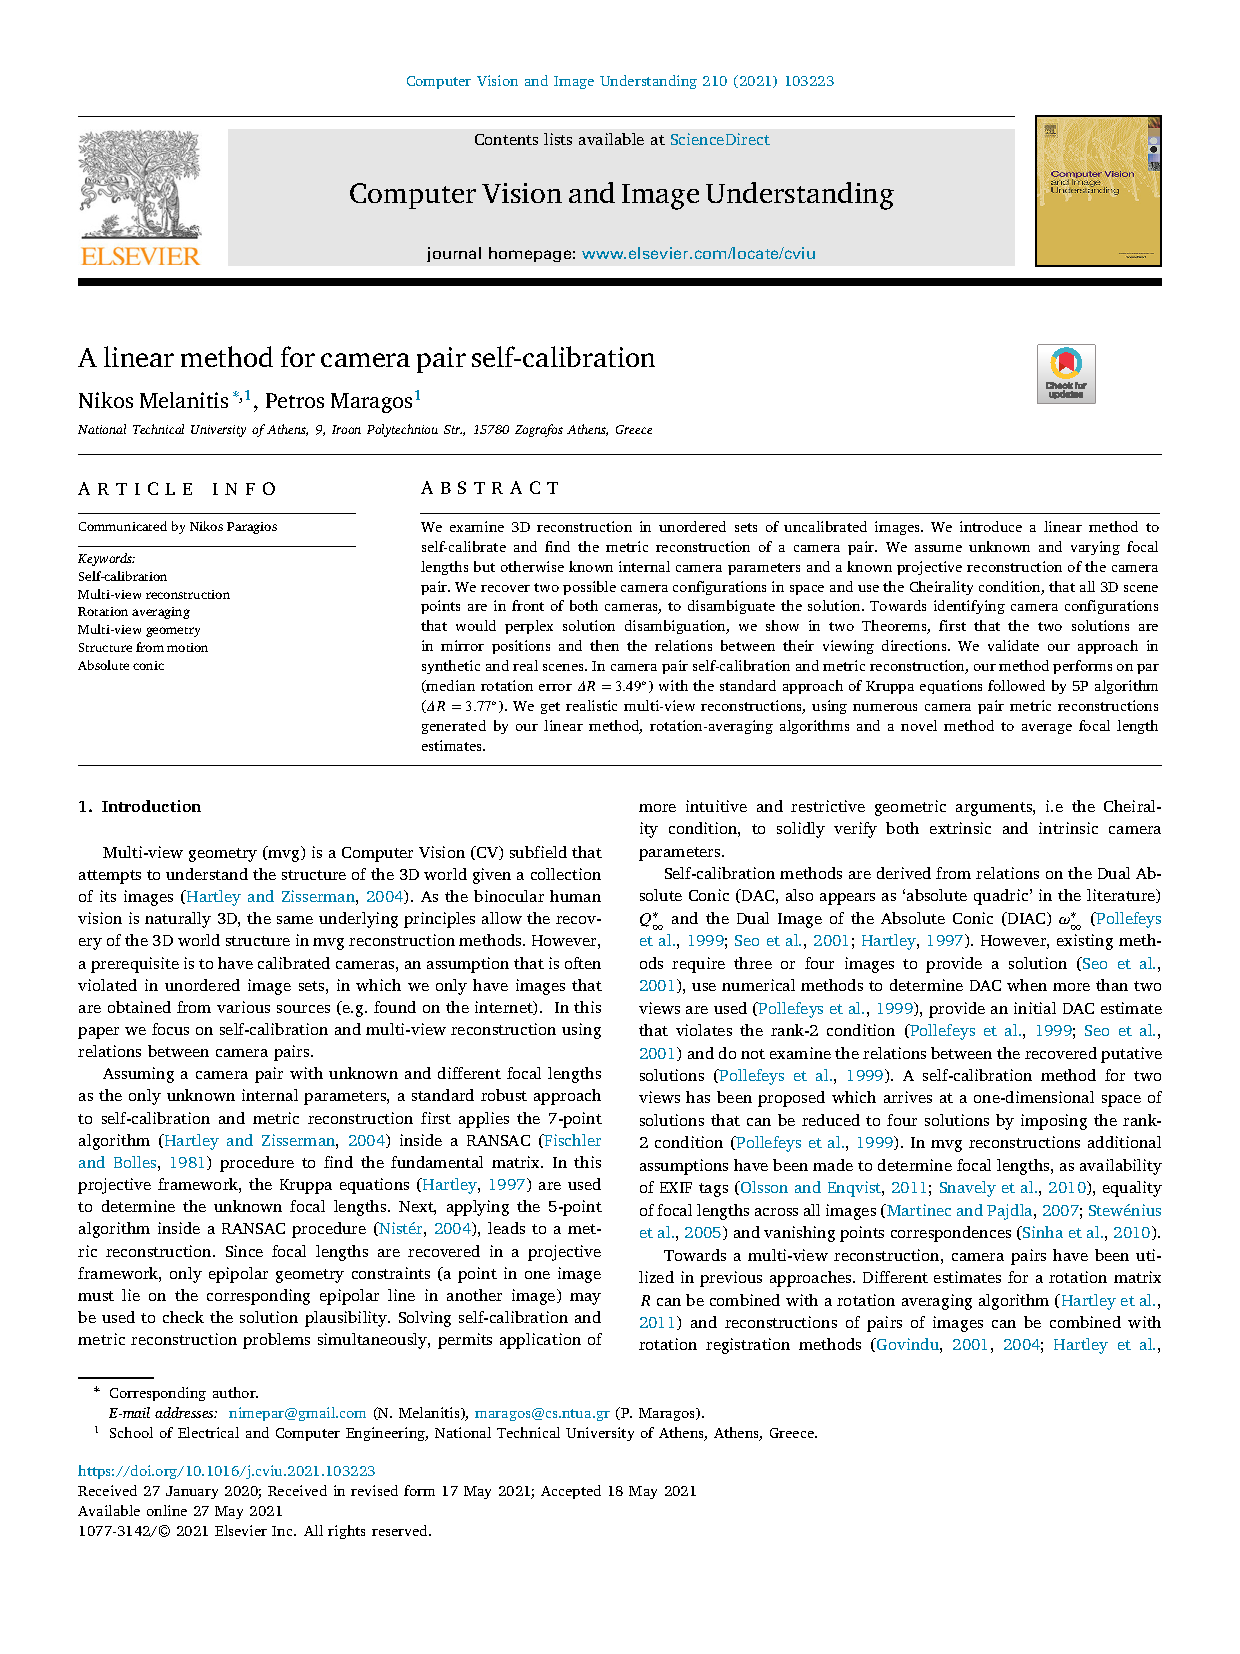
\includepdf[
	pages=-, % toutes les pages
	link=true, % permet de faire des hyperliens vers des pages en particulier
	linkname=article1, % pour les hyperliens, nom plus facile à manipuler
	addtotoc={
		1, section, 2, Titre original de l'article, sec:Article1,			%  item 1 Ne conserver que cet item dans le niveau  "section"
		2, subsection, 2, Background and related work, sec:AAA,    % item 2, page 2
		3, subsubsection, 4, A method for metric, sec:CCC,					% entree 3 non dans la TdM car on ne conserve que les étages 1 et 2
		4, subsection, 2, Recovering the solutions, subsec:BBB}	 % entree 4, page 4
]
{contenu/article.pdf} % nom et emplacement du fichier

%%%%%%%%%%%%%%%%%%%%%%%%%%%%%%%%%%%%%
% format de l'option addtotoc pour ajouter des éléments de l'article dans la table des matières. Ne pas en abuser.
%addtotoc={⟨page number ⟩,⟨section ⟩,⟨level ⟩,⟨heading ⟩,⟨label ⟩}
%⟨page number ⟩: Page number of the inserted page.
%⟨section⟩: LATEX sectioning name – e.g., section, subsection, . . .
%⟨level ⟩: Number, denoting depth of section – e.g., 1 for section level, 2 for subsection level, . . . si le niveau est plus grand que la prof. de la TOC (par défaut 2), aucun numéro n'apparait
%⟨heading⟩: Title inserted in the table of contents.
%⟨label ⟩: Name of the label. This label can be referred to with \ref and \pageref.

\section{Conclusion ou sections supplémentaires}

Rien n'empêche de conclure à part dans la langue principale du document. 

Possible de renvoyer à une page de l'article inséré à partir de n'importe où dans le document, comme suit :
\hyperlink{article1.5}{page 5} de l'article.

\Secref{CCC}.

Page \pageref{subsec:BBB} % fichier articlePublie.tex
	
	%=========================== CHAPITRE 3 ============================
	
	\modeDefaut
        \chapter[Modèle de Riesz]{Étude théorique du modèle de Riesz} % signal monogénique ?
\label{chap:chapitre3}

Dans le but de synthétiser du contenu avec de la structure irrégulière, nous cherchons à avoir une approche locale. Pour cela nous utilisons le modèle du signal monogénique \cite{felsberg_monogenic_2001}, qui permet d'extraire l'énergie locale, en s'appuyant sur la transformée de Riesz. Ce SY procédé est ensuite mis en application dans un cadre multi-résolutionnel, les pyramides de Riesz \cite{wadhwa_riesz_2014}, pour calculer la congruence de phases.

\section{Signal monogène}

Le signal monogène est un outil du domaine du traitement du signal, généralement utilisé pour des tâches d'analyse d'image ou de vision par ordinateur, comme la détection de caractéristiques. La revue de la méthode par Bridge \cite{bridge_introduction_2018} est une bonne introduction aux principes théoriques du signal monogène ; nous reprennons dans cette partie sa notation et son discours exposé dans son document afin de prodiguer une compréhension du modèle.

\subsection{Une dimension, signal analytique}

\subsubsection{Construction du singal analytique}

Pour comprendre l'utilité du signal monogène, commençons par expliquer le fonctionnement du signal analytique, dont le signal monogène est l'extension aux signaux de dimension arbitraire. Le signal analytique est une méthode de représentation d'un signal 1D à valeurs réelles, qui facilite la manipulation et l'extraction de certaines informations du signal original. Le constat qui donne lieu à cette représentation est que pour un signal à valeurs réelles, les fréquences négatives sont superflues pour sa représentation de Fourier. En effet, on rappelle que la transformée de Fourier $F(\omega)$ d'un signal à valeurs réelles $f(t)$ présente une symétrie hermitienne :

\begin{equation}
    F(-\omega) = \overline{F(\omega)}
\end{equation}

avec $\overline{\cdot}$ l'opérateur de conjugaison complexe. L'idée est donc de se débarrasser des fréquences négatives, sans perte d'information, et de construire un nouveau signal en n'utilisant que les fréquences positives de $f(t)$. On exprime d'abord le signal $F_{\alpha}$ dans le domaine de Fourier :

\begin{equation}
    F_{\alpha}(\omega) = \left\{
    \begin{array}{ll}
        2F(\omega), & \omega > 0 \\
        0, & \omega < 0 \\
        F(0), & \omega = 0,
    \end{array}
    \right.
\end{equation}

où l'amplitude des composantes de fréquences positives est doublée, par soucis de conservation d'énergie. Avec cette formulation, toute l'information de notre signal original est conservée, mais cette nouvelle forme permet de faire des manipulations précédemment impossibles qui nous permettent de mieux comprendre notre signal.

\begin{figure}[h]
    %\noindent
    \hspace{-12pt}
    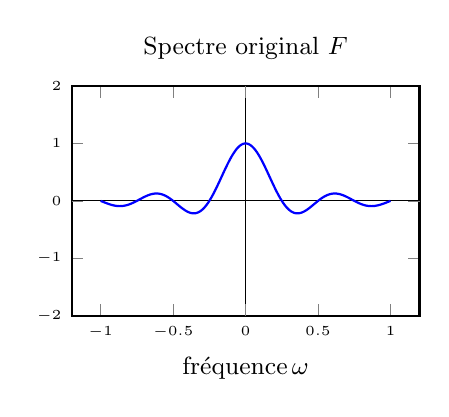
\begin{tikzpicture}
    \begin{axis}[
        title={Spectre original $F$},
        title style={font=\small},
        axis lines=box,
        style=thick,
        xlabel=\(\textnormal{fréquence}\, \omega\),
        xtick={-1, -0.5, 0.5, 1},
        ytick={-2, -1, 1, 2},
        extra x ticks=0,
        extra y ticks=0,
        extra x tick style={grid=major, grid style={black}},
        extra y tick style={grid=major, grid style={black}},
        tick label style={font=\tiny},
        label style={font=\small},
        ymin=-2, 
        ymax=2,
        ]
    \addplot[
        color=blue,
        domain=-1:1,
        samples=200
        ]
    {sin(360*x*2)/ (2*pi*x*2)};
    \end{axis}
    \end{tikzpicture}
    %\hskip 6pt
    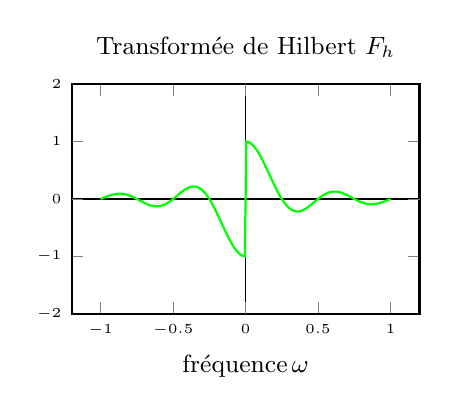
\begin{tikzpicture}
    \begin{axis}[
        title={Transformée de Hilbert $F_h$},
        title style={font=\small},
        axis lines=box,
        style=thick,
        xlabel=\(\textnormal{fréquence}\, \omega\),
        xtick={-1, -0.5, 0.5, 1},
        ytick={-2, -1, 1, 2},
        extra x ticks=0,
        extra y ticks=0,
        extra x tick style={grid=major, grid style={black}},
        extra y tick style={grid=major, grid style={black}},
        tick label style={font=\tiny},
        label style={font=\small},
        ymin=-2, 
        ymax=2,
        ]
    \addplot[
        color=green,
        domain=-1:1,
        samples=200
        ]
    {sign(x)*sin(360*x*2)/ (2*pi*x*2)};
    \end{axis}
    \end{tikzpicture}
    %\hskip 6pt
    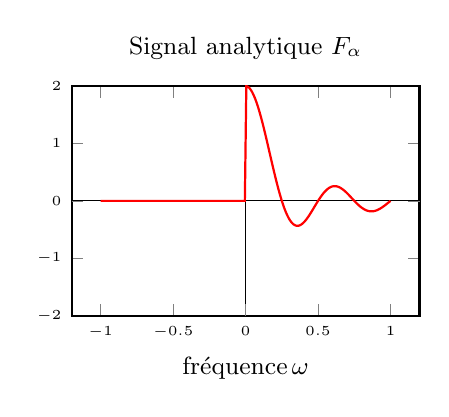
\begin{tikzpicture}
    \begin{axis}[
        title={Signal analytique $F_{\alpha}$},
        title style={font=\small},
        axis lines=box,
        style=thick,
        xlabel=\(\textnormal{fréquence}\, \omega\),
        xtick={-1, -0.5, 0.5, 1},
        ytick={-2, -1, 1, 2},
        extra x ticks=0,
        extra y ticks=0,
        extra x tick style={grid=major, grid style={black}},
        extra y tick style={grid=major, grid style={black}},
        tick label style={font=\tiny},
        label style={font=\small},
        ymin=-2, 
        ymax=2,
        ]
    \addplot[
        color=red,
        domain=-1:1,
        samples=200
        ]
    {(1+sign(x))*sin(360*x*2)/ (2*pi*x*2)};
    \end{axis}
    \end{tikzpicture}

    \captionof{figure}{Création du signal analytique dans le domaine fréquentiel (seule la partie réelle est montrée). Le signal original réel (gauche), qui présente une symétrie hermitienne, est ajouté à sa transformée de Hilbert (milieu), lui impair, pour former le signal analytique (droite), dépourvu de fréquence négative.}
    \label{fig:complex-analytic-representation}
\end{figure}

En effet, on peut voir le fait de supprimer les composantes de fréquences négatives comme le l'ajout d'un signal impair soigneusement choisi au signal de base.

\begin{equation} \label{eq:2.1}
    F_{\alpha}(\omega) = F(\omega) + F_h(\omega),
\end{equation}

où $F_h(\omega)$ est la « version impaire » du signal $F(\omega)$ :

\begin{equation}
    F_h(\omega) = \left\{
    \begin{array}{ll}
        F(\omega), & \omega > 0 \\
        -F(\omega), & \omega < 0 \\
        0, & \omega = 0,
    \end{array}
    \right.
\end{equation}

que l'on peut reformuler à l'aide de la fonction signe $\sgn$ :

\begin{equation}
    F_h(\omega) = F(\omega)\cdot \sgn(\omega).
\end{equation}

On rappelle l'expression de la fonction signe :

\begin{equation}
    \sgn(x) = \left\{
    \begin{array}{ll}
        1, & x > 0 \\
        -1, & x < 0 \\
        0, & x = 0.
    \end{array}
    \right.
\end{equation}

On obtient alors la ré-écriture de l'équation \ref{eq:2.1} :

\begin{equation}
    F_{\alpha}(\omega) = (1+\sgn(\omega))F(\omega)
\end{equation}

\begin{figure}[h]
    %\noindent
    %\hspace{-10pt}
    \centering
    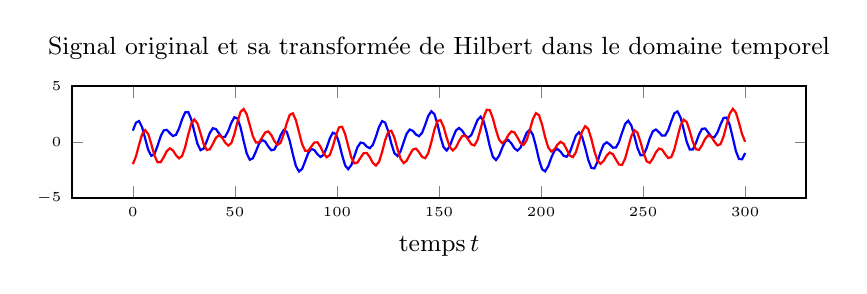
\begin{tikzpicture}
    \begin{axis}[
        title={Signal original et sa transformée de Hilbert dans le domaine temporel},
        title style={font=\small},
        axis lines=box,
        width=0.9\textwidth,
        height=3cm,
        style=thick,
        xlabel=\(\textnormal{temps}\, t\),
        xtick={0, 50, 100, 150, 200, 250, 300},
        ytick={-5, 0, 5},
        tick label style={font=\tiny},
        label style={font=\small},
        ymin=-5, 
        ymax=5,
        ]
    \addplot[
        color=blue,
        domain=0:300,
        samples=200
        ]
    {sin(3*x)+cos(15*x)+sin(30*x)};
    \addplot[
        color=red,
        domain=0:300,
        samples=200
        ]
    {-cos(3*x)+sin(15*x)-cos(30*x)};
    \end{axis}
    \end{tikzpicture}

    \captionof{figure}{Exemple de représentation analytique. Le signal original réel (en bleu), et sa transformée de Hilbert imaginaire pure (en rouge).}
    \label{fig:analytic-representation}
\end{figure}


Le signal $F_{\alpha}$ créé est donc dans le domaine fréquentiel de $F$, signal original pair, de représentation purement réelle dans le domaine temporel, et de $F_h$, signal impair, de représentation purement imaginaire dans le domaine temporel, que l'on nomme $f_h$. Dans le domaine temporel, $f_{\alpha}$ est donc un signal complexe, sans composantes de fréquences négatives, c'est un signal analytique, que l'on appelle la \textit{représentation analytique} de $f$ :

\begin{equation}
    f_{\alpha}(t) = \underbrace{f(t)}_\text{réel pur} + \underbrace{f_h(t)}_\text{imaginaire pur}.
\end{equation}

Le signal ajouté pour annuler les fréquences $F_h$ est par ailleurs un objet connu : c'est la \textit{transformée de Hilbert} de $F$. Sa représentation, bien que très simple dans le domaine fréquentiel, est difficile à obtenir et manipuler dans le domaine temporel :

\begin{equation}
    f_h(t) = i \cdot \textnormal{p.v.} \int_{-\infty}^{\infty} \frac{f(t)}{\pi(t-\tau)} \,d\tau,
\end{equation}

où p.v. est la valeur principale de Cauchy, nécessaire pour cette intégrale, qui représente la convolution avec la distribution $\frac 1{\pi t}$ et qui est impropre à cause de la singularité en $t=\tau$. Cependant, dû à la complexité de cet objet, nous utiliserons majoritairement l'expression fréquentielle de la transformée de Hilbert :

\begin{align*}
    &\hil(F) = F_h = \sgn\cdot F \\
    &\mathcal{H}(F) = F_h = \sgn\cdot F
\end{align*}


\subsubsection{Amplitude et phase locales}

Pour comprendre l'intérêt du signal analytique, on étudie d'abord l'exemple d'une fonction sinusoïdale, d'amplitude $A$ et de fréquence $\omega_0$ fixées :

\begin{equation}
    f(t) = A\sin(\omega_0t).
\end{equation}

En utilisant les relations montrées précédemment, on trouve la transformée de Hilbert de $f$ et on calcule sa représentation analytique :

\begin{align}
    f_h(t) &= iA\cos(\omega_0t) \\
    f_{\alpha}(t) &= f(t) + f_h(t) \\
    &= A\sin(\omega_0t)+iA\cos(\omega_0t) \\
    &= Ae^{i\omega_0t}.
\end{align}

Pour une sinusoïde, la transformée de Hilbert est un simple \textit{déphasage} de $-\frac{\pi}2$ du signal original. Or la théorie de Fourier nous indique que n'importe quel signal générique peut être décomposé comme une somme de sinusoïdes. Ainsi la transformée de Hilbert agit de la même manière sur tous les signaux : c'est un déphasage de $-\frac{\pi}2$ de chaque composante fréquentielle qui compose le signal. Le signal $f$ et sa transformée de Hilbert $f_h$ sont dit en \textit{quadrature de phase}, et le signal analytique s'exprime comme une exponentielle complexe.

\bigskip

En fait, puisque tout signal est maintenant représenté comme la somme d'un réel et d'un imaginaire pur, on peut toujours l'exprimer en coordonnées polaires comme une exponentielle complexe, d'amplitude et phase variant au cours du temps :

\begin{equation}
    f_{\alpha} (t) = A(t)e^{i\phi(t)}.
\end{equation}

avec 

\begin{align}
    A(t) &= \sqrt{f(t)^2 + h_h(t)^2} \\
    \phi(t) &= \arctan\left(\frac{f_h(t)}{f(t)}\right).
\end{align}

Cette représentation introduit le concept d'\textit{amplitude locale} et de \textit{phase locale} (ici \textit{temporellement} locales), qui sont deux outils d'analyse particulièrement intéressants pour l'étude approfondie du signal original. L'amplitude locale agit comme une mesure de l'\textit{enveloppe} du signal, et la phase locale comme une mesure de la \textit{forme} du signal. Par exemple, une phase de $0$ indique un extremum, et une phase de $\pm\pi$ indique un passage par zéro. La figure \ref{fig:local-pha-amp} montre un signal avec son amplitude locale et sa phase locale. À partir uniquement de notre signal initial, on a ainsi créé un outil nous permettant d'obtenir de l'information bien plus intéressante sur l'apparence et les propriétés du signal.

\begin{figure}[h]

    \centering
    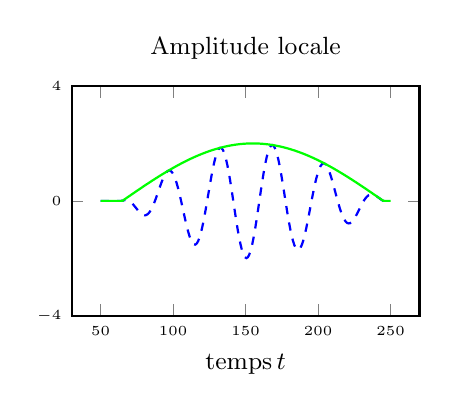
\begin{tikzpicture}
    \begin{axis}[
        title={Amplitude locale},
        title style={font=\small},
        axis lines=box,
        %width=0.9\textwidth,
        %height=3cm,
        style=thick,
        xlabel=\(\textnormal{temps}\, t\),
        xtick={50, 100, 150, 200, 250},
        ytick={-4, 0, 4},
        tick label style={font=\tiny},
        label style={font=\small},
        ymin=-4, 
        ymax=4,
        ]
    \addplot[
        color=blue,
        domain=50:250,
        samples=200,
        style=dashed,
        ]
    {(sign(x-65)-sign(x-245))*sin(10*x+25)*cos(x+25)};
    \addplot[
        color=green,
        domain=50:250,
        samples=200
        ]
    {(sign(x-65)-sign(x-245))*sqrt((0.5*(sin(11*x-40) + sin(9*x-90)))^2 + (sin(10*x+25)*cos(x+25))^2)};
    \end{axis}
    \end{tikzpicture}
    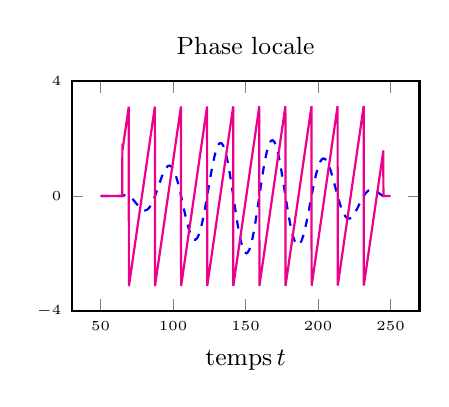
\begin{tikzpicture}
    \begin{axis}[
        title={Phase locale},
        title style={font=\small},
        axis lines=box,
        %width=0.9\textwidth,
        %height=3cm,
        style=thick,
        xlabel=\(\textnormal{temps}\, t\),
        xtick={50, 100, 150, 200, 250},
        ytick={-4, 0, 4},
        tick label style={font=\tiny},
        label style={font=\small},
        ymin=-4, 
        ymax=4,
        ]
    \addplot[
        color=blue,
        domain=50:250,
        samples=200,
        style=dashed,
        ]
    {(sign(x-65)-sign(x-245))*sin(10*x+25)*cos(x+25)};
    \addplot[
        color=magenta,
        domain=50:250,
        samples=2000
        ]
    {(sign(x-65)-sign(x-245))*rad(atan((0.5*(sin(11*x-40) + sin(9*x-90))) / (sin(10*x+25)*cos(x+25))))};
    \end{axis}
    \end{tikzpicture}

    \caption{Extraction d'informations locales pour un cosinus modulé par un sinus. L'amplitude locale (gauche) donne l'enveloppe de la sinusoïde, et la phase locale (droite) nous donne de l'information quant à la position dans le cycle d'oscillation.}
    \label{fig:local-pha-amp}

\end{figure}

\subsubsection{Notion d'échelle}

L'exemple donné avec la figure \ref{fig:local-pha-amp} fonctionne bien car le signal est simple, l'interprétation de l'amplitude et la phase locale est claire et visuelle. Pour un signal plus complexe, plus représentatif des signaux que l'on doit souvent étudier, ce n'est pas si facile. La figure \ref{fig:complex-local-pha-amp} affiche les informations locales du signal de la figure \ref{fig:analytic-representation}, une somme de trois sinusoïdes de fréquences différentes ; il est moins évident de comprendre ce que les informations locales représentent dans ce cas.

\begin{figure}[h]
    \centering
    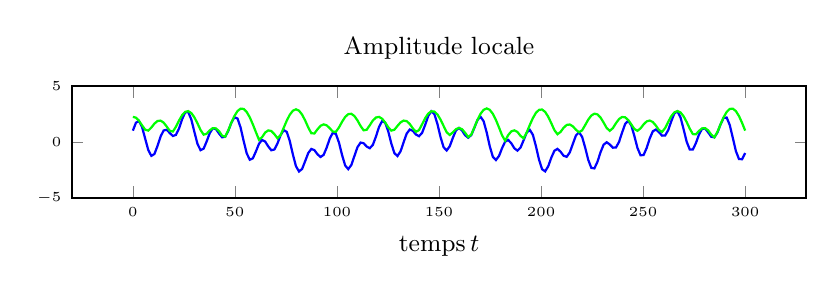
\begin{tikzpicture}
    \begin{axis}[
        title={Amplitude locale},
        title style={font=\small},
        axis lines=box,
        width=0.9\textwidth,
        height=3cm,
        style=thick,
        xlabel=\(\textnormal{temps}\, t\),
        xtick={0, 50, 100, 150, 200, 250, 300},
        ytick={-5, 0, 5},
        tick label style={font=\tiny},
        label style={font=\small},
        ymin=-5, 
        ymax=5,
        ]
    \addplot[
        color=blue,
        domain=0:300,
        samples=200
        ]
    {sin(3*x)+cos(15*x)+sin(30*x)};
    \addplot[
        color=green,
        domain=0:300,
        samples=200
        ]
    {sqrt((sin(3*x)+cos(15*x)+sin(30*x))^2 + (-cos(3*x)+sin(15*x)-cos(30*x))^2)};
    \end{axis}
    \end{tikzpicture}
    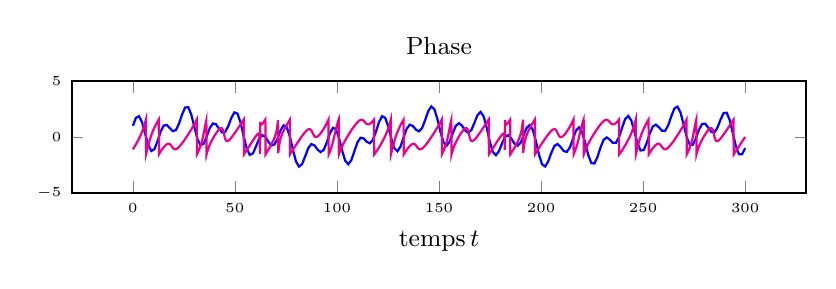
\begin{tikzpicture}
    \begin{axis}[
        title={Phase},
        title style={font=\small},
        axis lines=box,
        width=0.9\textwidth,
        height=3cm,
        style=thick,
        xlabel=\(\textnormal{temps}\, t\),
        xtick={0, 50, 100, 150, 200, 250, 300},
        ytick={-5, 0, 5},
        tick label style={font=\tiny},
        label style={font=\small},
        ymin=-5, 
        ymax=5,
        ]
    \addplot[
        color=blue,
        domain=0:300,
        samples=200
        ]
    {sin(3*x)+cos(15*x)+sin(30*x)};
    \addplot[
        color=magenta,
        domain=0:300,
        samples=3000
        ]
    {rad(atan((-cos(3*x)+sin(15*x)-cos(30*x)) / (sin(3*x)+cos(15*x)+sin(30*x))))};
    \end{axis}
    \end{tikzpicture}    

    \caption{Caption}
    \label{fig:complex-local-pha-amp}
\end{figure}

Le problème à l'analyse de ce signal est le fait qu'il existe plusieurs niveaux de structure, qui interfèrent et rendent l'interprétation des informations locales impossible à l'échelle macroscopique.
Pour extraire de l'information utile, il faut sélectionner et faire l'analyse d'un seul niveau de structure, donc d'échelle.
Pour cela, on filtre les composantes des niveaux qui ne nous intéressent pas.
Pour se faire, il est possible d'utiliser des filtres passe-bande, comme le fait Bridge avec les filtres log-Gabor, un choix commun pour ce genre de pratique.
Un filtre log-Gabor est un filtre défini dans le domaine fréquentiel, qui permet de sélectionner une bande de fréquence centrée autour d'une fréquence centrale $\omega_0$.
Il a une réponse en fréquence de forme gaussienne quand observé en échelle logarithmique :

\begin{equation}
    G(\omega) = \exp\left(-\frac{\log^2(\frac{|\omega|}{\omega_0})}{2\log(\sigma_0)^2}\right).
\end{equation}

Ces filtres sont caractérisés par deux paramètres : la fréquence centrale $\omega_0$, qui contrôle quelle échelle de structure est sélectionnée, et la largeur de bande $\sigma_0$, un paramètre de forme qui contrôle la largeur de la bande de fréquence sélectionnée. Des exemples de filtre log-Gabor sont montrés à la figure \ref{fig:log-gabor-filters}.

En appliquant un filtre log-Gabor à notre signal avant de lui appliquer la transformée de Hilbert et de déterminer sa représentation analytique, on obtient une représentation locale du signal, centrée autour d'une fréquence $\omega_0$ et d'une échelle $\sigma_0$ que l'on peut faire varier arbitrairement.

\begin{equation}
    F_{\alpha}(\omega) = (1+\sgn(\omega))G(\omega)F(\omega)
\end{equation}

\begin{figure}
    \centering
    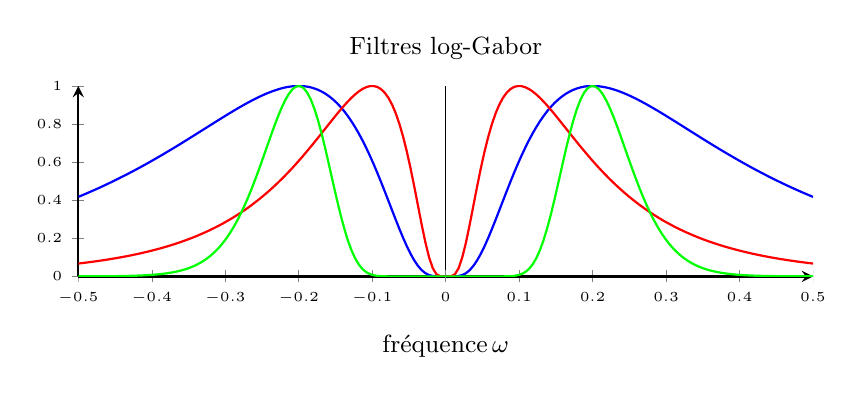
\begin{tikzpicture}
    \begin{axis}[
        title={Filtres log-Gabor},
        title style={font=\small},
        axis lines=left,
        width=0.9\textwidth,
        height=4cm,
        style=thick,
        xlabel=\(\textnormal{fréquence}\, \omega\),
        xtick={-0.5, -0.4, -0.3, -0.2, -0.1, 0.1, 0.2, 0.3, 0.4, 0.5},
        ytick={0, 0.2, 0.4, 0.6, 0.8, 1},
        tick label style={font=\tiny},
        label style={font=\small},
        extra x ticks=0,
        extra x tick style={grid=major, grid style={black}},
        ymin=0,
        ymax=1,
        ]
    \addplot[
        color=blue,
        domain=-0.5:0.5,
        samples=200
        ]
    {exp(-ln(abs(x)/.2)^2 / (2*ln(.5)^2))};
    \addplot[
        color=red,
        domain=-0.5:0.5,
        samples=200
        ]
    {exp(-ln(abs(x)/.1)^2 / (2*ln(.5)^2))};
    \addplot[
        color=green,
        domain=-0.5:0.5,
        samples=200
        ]
    {exp(-ln(abs(x)/.2)^2 / (2*ln(.8)^2))};
    \end{axis}
    \end{tikzpicture}

    \caption{Représentation dans le domaine fréquentiel de filtres log-Gabor de différents paramètres. En rouge, $\omega_0=0.1, \sigma_0 = 0.5$. En bleu, $\omega_0=0.2, \sigma_0 = 0.5$. En vert, $\omega_0=0.2, \sigma_0 = 0.8$.}
    \label{fig:log-gabor-filters}
\end{figure}

En étudiant la réponse du signal sur une large gamme de fréquences et d'échelles, on obtient une représentation locale du signal à différentes échelles, et ainsi extraire de l'information sur les différentes structures du signal. On peut rassembler toutes ces informations dans un graphique appelé scalogramme, qui représente le comportement de la phase locale en fonction du temps et de l'échelle, comme montré à la figure~\ref{fig:scalogram}. On y voit facilement les différents niveaux de structure du signal, et l'interprétation des informations locales devient plus utile car on peut choisir à quel niveau on regarde.

Si l'on compare le modèle du signal analytique à celui de la transformée de Fourier, on remarque que les informations que l'on obtient avec les deux diffèrent et se complètent. La transformée de Fourier nous donne de l'information globale sur tout le signal, mais localisée en termes de fréquence. La représentation analytique, elle, nous donne une information spatialement locale sur le signal, mais sur une bande de fréquences, sélectionnées par un filtre passe-bande. Le modèle d'information locale est donc un compromis entre la localisation spatiale et fréquentielle, et permet d'obtenir une information différente sur le signal.


\begin{figure}
    \centering
    \includegraphics[width=\textwidth]{contenu/resources/images/scalogram}
    \caption{Scalogramme de la phase locale pour un signal complexe. La phase locale est représentée en échelle de gris, et varie en fonction du temps (en abscisse) et de l'échelle en nombre de pixels (en ordonnée). Diagramme par Bridge~\cite{bridge_introduction_2018}.}
    \label{fig:scalogram}
\end{figure}


\subsection{Deux dimensions, signal monogène}

Le modèle du signal analytique est utile à l'extraction d'informations locales pour des signaux 1D, et il serait intéressant d'avoir accès à ces informations pour des images, donc des signaux 2D. En effet l'importance de la phase dans l'analyse d'image a déjà été soulignée depuis longtemps~\cite{oppenheim_importance_1981}. Cependant, l'application n'est pas directe dans le cas de deux (ou plus) dimensions, car il y a une notion de direction à considérer. C'est ce que le modèle du signal monogène, proposé par Felsberg et Sommer~\cite{felsberg_monogenic_2001}, permet de faire, que nous allons développer dans cette partie.

\subsubsection{Construction du signal monogène}



\section{Transformée de Riesz}

\section{Pyramide de Riesz}

	%\chapter[Article soumis ou en préparation]
{Titre long en français d'un chapitre contenant un article soumis ou en préparation}
\label{chap:soumis}

\begin{authorsArticle} % dans l'ordre de la publication
	\begin{description}
		\item[\large nom 1] Affiliation
		\item[\large nom 2] Affiliation
		\item[\large ...] 
	\end{description}
\end{authorsArticle}
%\authorArticle{
	%}

\begin{abstractArticle}
	Résumé de l'article en français. Ce résumé peut être la traduction de l'article s'il est en anglais.
\end{abstractArticle}
% resumeArticle{}

\begin{contributions}
	Décrivez dans cette section les contributions de l'article.
\end{contributions}

\begin{commentairesArticle}
	Décrivez dans cette section la part de chacun.e des auteur.e.s
\end{commentairesArticle}

% - choisir la bonne option parmi les deux suivantes
\modeAnglais
%\modeFrancais
% --------------------------------------------

% IMPORTANT : ARTICLE TEL QUE SOUMIS
\titleArticle{Titre de l'article soumis}

\keywordsArticle{ keywords }

Intro de l'article ...

\section{Section Title }

Vous devez introduire la section.

\subsection{Sub-section Title}

Vous devez introduire la  sous-section.

\subsection{Sub-section Title}

Vous devez introduire la  sous-section.

\subsubsection{Sub-sub-section Title}

Vous devez introduire la  sous-sous-section.

\paragraph{A paragraph:} example

\subparagraph{A sub-paragraph:} exemple

\subsubsection{Sub-sub-section Title}

Vous devez introduire la  sous-sous-section.

\subsection{Sub-section Title}

Vous devez introduire la  sous-section.
 % fichier articleSoumis.tex

        \modeDefaut
        \chapter{Implémentation et échange de contenu variable}
\label{chap:chapitre4}

\section{Outils de développement}

\subsection{Détails d'implémentation}
- choix du filtre pour la pyramide de Gauss / Laplace
- approximation de la transformée de Riesz par le gradient

\subsection{OpenCV}
\subsection{Godot 3.x}
\subsection{Godot 4.0}
\subsection{TexSyn}

\section{Visualisation de la congruence de phase}

\section{Sélection de niveaux de fréquences précis et applications}

\subsection{Application à l'échange de contenu de PC variable}

\subsection{Filtrage de bande de basse fréquence}

\section{Synthèse de texture préservant la congruence de phase}

\subsection{Synthèse par ré-organisation}

\subsection{Échantillonneur préservant la congruence de phase}

 
	%=========================== CONCLUSION ============================

	\modeDefaut
	\Conclusion \label{chap:conclusion}

% MF CORRECTION DONE

Le travail dont ce mémoire fait l'objet est une étude exploratoire du cadre de travail local multirésolution mis au point en utilisant la transformée de Riesz. D'habitude utilisés dans le domaine du traitement du signal, ces outils sont ici examinés pour faire l'analyse de textures présentant des structures irrégulières, textures qui sont encore aujourd'hui en enjeu non résolu du domaine de la synthèse de texture procédurale~\cite{guehl_semi-procedural_2020}. Le but de cette étude est de voir si de tels outils peuvent aider à résoudre, au moins partiellement, le problème de la synthèse de texture procédurale de textures à structure irrégulière.

\bigskip

Une mise en contexte et exposition au domaine et à la problématique de la synthèse de texture à structure irrégulière est faite en introduction~\ref{chap:introduction}. Quelques approches existantes y sont présentées et des notions nécessaires à la compréhension du problème sont abordées. Un aperçu plus approfondi des méthodes employées dans ce travail est donné dans un second temps au chapitre~\ref{chap:chapitre1}. La théorie du signal monogène utilisant la transformée de Riesz est présentée, en mettant l'accent sur le concept d'information locale à extraire d'une image et la signification qui peut lui être attribuée. La description de l'outil d'analyse local multirésolution des pyramides d'images de Riesz est ensuite faite, en détaillant les différentes étapes de construction et choix d'implémentation. Enfin la fonction de congruence de phases issue du modèle d'énergie locale de Morrone \textit{et al.}~\cite{morrone_feature_1987, morrone_mach_1986} et son importance pour l'analyse de la structure d'une image sont discutées. Une méthode de calcul adaptée au cadre de travail choisi est aussi proposée. Dans un dernier temps, les différentes applications de ces outils sont présentées au chapitre~\ref{chap:chapitre2}. La décomposition en pyramide d'images permet la mise en place d'une méthode de sélection fréquentielle du contenu d'une image, utilisée pour faire du gommage de contenu indésirable dans des textures. Un échantillonneur préférentiel préservant la congruence de phases, inspiré de Pharr \textit{et al.}~\cite{pharr_physically_2023}, est ensuite dérivé et mis en application dans une méthode de synthèse de texture, pour tenter de synthétiser du contenu à structure irrégulière. Les résultats obtenus et les limites de notre approche sont discutées à la suite de cela.

\bigskip

Finalement, quelques perspectives de travaux futurs et pistes d'améliorations, relevées lors de cette étude, sont ici proposées. Une continuation de ce travail serait de s'intéresser à l'orientation locale qui découle du signal monogène. Cette grandeur a en effet été mise de côté dans cette étude pour se concentrer sur la phase, mais elle pourrait être utilisée comme information supplémentaire pour guider la synthèse de texture. Il a été discuté que la congruence de phases seule n'était pas suffisante pour bien préserver les éléments de structure d'une texture~\ref{par:discussion-synthesis}, l'utilisation de l'orientation est une piste à explorer pour complémenter la congruence. Reinhardt \textit{et al.}~\cite{reinhardt_multi-scale_2022} ont d'ailleurs montré que l'orientation extraite du signal monogène à l'aide de la transformée de Riesz est un bon outil pour certaines tâches de traitement d'image comme la détection d'orientation d'éléments ou la détection de défauts dans un tissu. Pour continuer dans la direction d'une synthèse capable de traiter des textures à structure irrégulière, travailler à mieux préserver des corrélations locales entre les pixels des textures serait pertinent. Plusieurs méthodes de la littérature s'intéressent à ce problème~\cite{cavalier_local_2019, heitz_high-performance_2018}, intégrer l'échantillonneur mis au point dans ce travail à ces travaux pourrait donner lieu à une méthode moins expérimentale et plus employable en pratique. Enfin toujours dans cette optique, la recherche de techniques de disposition de contenu pour la création de nouvelle structure lors de la synthèse reste un sujet ouvert. Sa résolution serait une grande avancée dans la synthèse de texture à structure irrégulière et donnerait lieu à des méthodes que notre échantillonneur pourrait bien complémenter.

	%=================================================================
	%=================== BIBLIOGRAPHIE  ======================
	%=================================================================
	
	%% Le style de la bibliographie peut être modifié ici
	% ce style pour une bibliographie en anglais
%	\include{style/UdeSDIengbst.tex}
%	\bibliographystyle{style/UdeSDIeng}
	
	
	% ce style pour une bibliographie en francais
	\bibliographystyle{style/UdeSDIfr}
	\include{style/UdeSDIfrbst}
	
	%% --- Bibliographie
	\bibliography{bibliographie} % fichier bibliographie.bib
	% Il est possible de mettre plusieurs noms de fichiers séparés par une virgule.
	\addcontentsline{toc}{chapter}{\bibname}

	%%=================================================================
	%%========================== ANNEXES ==============================
	%%=================================================================
	
%	\appendix
	
	%% Les annexes peuvent \^etre en fran\c{c}ais ou en anglais
	%% Si elles sont en anglais dans un document français, elles doivent contenir \modeAnglais ou \englishMode
	%% juste après la commande \chapter{xxx}
	
	%%=========================== ANNEXE EXEMPLE ============================
	
%	\modeDefaut
%	\chapter{Utilisation de la bibliothèque TexSyn}
\label{app:texsyn-use}

La bibliothèque logicielle de synthèse de texture et de traitement d'image TexSyn est un outil de synthèse de texture procédurale développé en collaboration avec Nicolas Lutz, post-doctorant du laboratoire. Elle est disponible en ligne sur un dépôt Github à l'adresse suivante: \url{https://github.com/VivienGAGLIANO/godot} (fourche du projet initial de Nicolas Lutz). Une courte notice d'utilisation est ici présentée, afin de faciliter la prise en main de l'outil.

\section{Présentation et mise en place}

La bibliothèque développée est un module pour le logiciel Godot, moteur de jeu et logiciel libre. Un bref aperçu du développement pour Godot est décrit, puis la méthode d'installation de la bibliothèque est expliquée. Enfin quelques conseils d'utilisation sont fournis.

\subsection{Développement pour Godot}

Une force du moteur Godot, et un de ses aspects qui le rendent populaire notamment pour la recherche, est que le code source est accessible et facilement modifiable. Cet aspect participatif du développement du moteur fait d'ailleurs partie de la philosophie de Godot, qui est pensé pour être une base de code à laquelle les utilisateurs contribuent selon leurs besoins. L'implémentation de fonctionnalités pour Godot est donc facilitée par la structure du moteur, qui permet l'intégration de modules écrits en divers langages de programmation.

\bigskip

La bibliothèque TexSyn est développée en C++, pour des raisons de performances. L'objectif étant la mise au point de méthodes de synthèse en temps réel, il est important que le code soit le plus rapide possible, le choix du langage C++ reflète ce désir. La bibliothèque est ensuite intégrée à Godot en tant que module, et les fonctionnalités de synthèse sont accessibles directement dans l'interface de Godot.

\subsection{Installation de la bibliothèque}

Pour intégrer TexSyn (ou tout autre module personnalisé) à un projet Godot, il est nécessaire de construire soit-même le moteur à partir du code source. Ce code source se trouve dans le dépôt Github mentionné au-dessus. Le code pour TexSyn se trouve dans la branche \texttt{texsyn4} du dépôt, qui est écrit pour Godot 4 (version 4.0 au moment du développement). Le processus d'installation et les détails de construction sont décrits en détail dans la \href{https://docs.godotengine.org/en/stable/contributing/development/compiling/index.html}{documentation} de Godot, mais un résumé des étapes importantes est donné ici.

\paragraph{Construction du logiciel}

Godot est développé en C++ et utilise SCons comme moteur de production. Il peut être construit pour plusieurs plateformes, celles utilisées lors du développement sont Linux et Windows. Lors de la compilation, il faut appeler le script SCons avec les options nécessaires pour spécifier la bonne plateforme et d'éventuels autres paramètres de compilation.

\paragraph{Compilation et édition de liens de TexSyn}

La bibliothèque TexSyn est implémentée comme une bibliothèque dynamique partagée. Une fois la compilation initiale du moteur faite, il est possible de modifier et compiler TexSyn sans avoir à recompiler tout le moteur (voir cette \href{https://docs.godotengine.org/en/stable/contributing/development/core_and_modules/custom_modules_in_cpp.html}{page de documentation} pour plus de détails). Pour cela, utiliser la variable d'environnement \texttt{texsyn\_shared=yes} et préciser la cible \texttt{bin/libtexsyn.linuxbsd.editor.dev.x86\_64.so} (nom pouvant différer légèrement selon la plateforme et les options de configurations sélectionnées) lors de la compilation. Pour que la bibliothèque soit accessible dans l'interface de Godot, il est aussi nécessaire que l'objet partagé créé soit accessible par le moteur. Il faut pour cela placer cet objet partagé avec l'exécutable du moteur créé, ou référencer son chemin d'accès, par exemple avec la variable d'environnement LD\_LIBRARY\_PATH sous Linux : \texttt{export LD\_LIBRARY\_PATH=\$PWD/bin/} depuis la racine du projet.

\paragraph{Ajout à la bibliothèque TexSyn}

Pour ajouter des fonctionnalités, classes ou fonctions à TexSyn, il faut suivre le \href{https://docs.godotengine.org/en/stable/contributing/development/core_and_modules/custom_modules_in_cpp.html}{procédé} décrit dans la documentation. Pour créer une nouvelle classe utilisable depuis un script Godot en GDScript (langage de script utilisé pour programmer la logique de jeu dans l'interface), il faut s'assurer que la classe hérite de \texttt{RefCounted}, inclure la commande \texttt{GDCLASS(NomDeMaClasse, RefCounted);} au début de la déclaration de la classe, définir et implémenter la méthode \texttt{\_bind\_methods()} pour lier les méthodes de la classe à l'interface de Godot, et enfin enregistrer la classe dans la liste des classes exportées dans le fichier \texttt{register\_types.cpp}. La classe et ses fonctions seront ensuite accessibles depuis l'interface. Plusieurs classes sont implémentées dans TexSyn et pourront servir d'exemple pour l'ajout de nouvelles fonctionnalités.

\section{Utilisation de TexSyn pour l'analyse et synthèse de texture}

Une fois le moteur et TexSyn construits, il est possible de créer un projet Godot et de commencer à utiliser les fonctions déjà implémentées. La personne intéressée trouvera un exemple de projet utilisant TexSyn pour implémenter des méthodes de base de synthèse procédurale de texture dans le dépôt Github suivant : \url{https://github.com/DrLutzi/godot-texsyn-scripts} (crédits à Nicolas Lutz pour ce projet). La scène d'exemple présente dans ce projet ne concerne par contre pas les travaux dont ce mémoire fait l'objet. L'utilisation de ces implémentations est ici brièvement décrite.

\paragraph{Construction de la pyramide de Riesz et calcul de la congruence de phases}

Pour construire la pyramide de Riesz d'une texture, la classe \texttt{RieszPyr} est utilisée. Cette classe comporte de nombreuses fonctions utiles à la construction et manipulation de la pyramide. La classe s'initialise avec la fonction \texttt{init}, en donnant en argument une \texttt{Image} qui contient les données d'une \texttt{Texture2D}. Les étages de la pyramide sont accessibles de manière unitaire à l'aide de la fonction \texttt{get\_layer}. Il est aussi possible de les récupérer tous à la fois, stockés dans un atlas de texture, avec la fonction \texttt{pack\_in\_texture}. Cette fonctionnalité est notamment utile lorsqu'il est nécessaire d'accéder à tous les niveaux de la pyramide simultanément depuis le \textit{fragment shader}. Enfin la congruence de phases est calculée à l'aide de la fonction \texttt{phase\_congruency}.

\paragraph{Utilisation de l'échantillonneur préférentiel}

Pour utiliser l'échantillonneur préférentiel et la méthode de synthèse discutés dans la section~\ref{sec:pc-preserving-synthesis}, la classe \texttt{RieszSampling} est utilisée. Les étapes à suivre sont l'extraction de la congruence de phases de l'exemple d'entrée (avec la classe \texttt{RieszPyr}) et sa quantification avec la méthode \texttt{quantize\_texture}, le partitionnement de la texture en différentes composantes (typiquement deux, les pavés et l'arrière-plan) avec \texttt{partition\_image}, et enfin le pré-calcul de la réalisation avec \texttt{precompute\_sampler\_realization}. Cette réalisation peut ensuite être chargée sur GPU comme un \texttt{Texture2DArray} pour être utilisée dans la synthèse qui se fait depuis le \textit{fragment shader}. % fichier annexe-A.tex
	
	%%=========================== ANNEXE PRÉCISIONS LATEX ============================
	
%	\modeDefaut
%	% !TeX spellcheck = fr_FR
%%%%%%%%%%%%%%%%%%%%%%%%%%%%%%%%%%%%%%%%%%%%%%%%%%%%%%%%%%%%
\chapter{Précisions sur Latex}
\label{chap:latex}
%%%%%%%%%%%%%%%%%%%%%%%%%%%%%%%%%%%%%%%%%%%%%%%%%%%%%%%%%%%%

L'annexe courante donne des exemples (voir fichier \texttt{annexes/annexe-SpecLatex.tex}) pour utiliser différents paquets inclus dans la classe. 

\section{Abbréviations et accronymes}
%%%%%%%%%%%%%%%%%%%%%%%%%%%%%%%%%%%%%%%%%%%%%%%%%%%%%%%%%%%%

....

\section{Figures}
%%%%%%%%%%%%%%%%%%%%%%%%%%%%%%%%%%%%%%%%%%%%%%%%%%%%%%%%%%%%


Une figure devrait être dans un environnement flottant et préférablement positionnée en haut ou en bas de page (option de positionnement \texttt{tb}) :

\begin{lstlisting}[nolol,numbers=none,frame=]
\begin{figure}[tb]
	\centering
	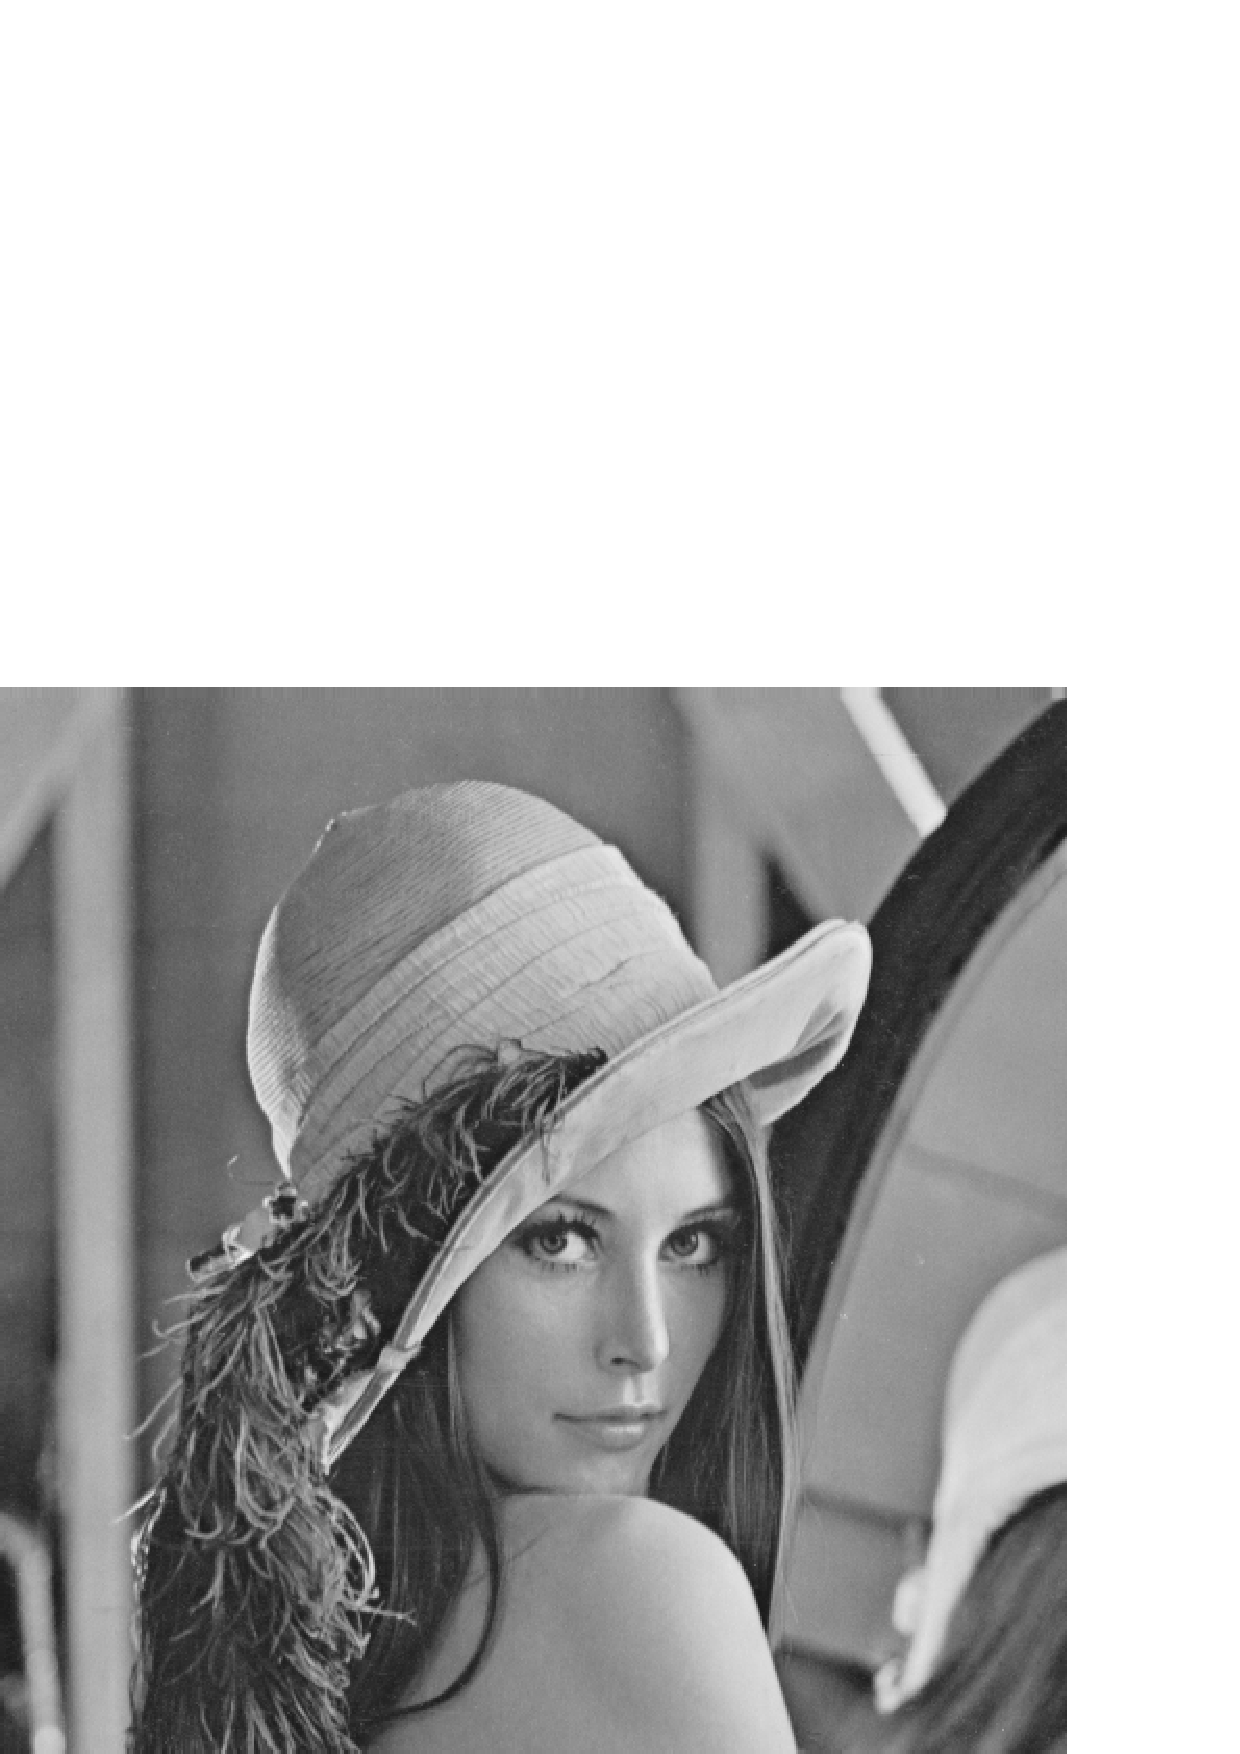
\includegraphics[width=0.45\linewidth]{lena.png}
	\caption[Titre pour la liste des figures]{On pourra mettre ce qu'on veut sous la figure, le titre dans la table des figures demeurera court.}
	\figlabel{figureSeule}
\end{figure}
\end{lstlisting}

\begin{figure}[tb]
	\centering
	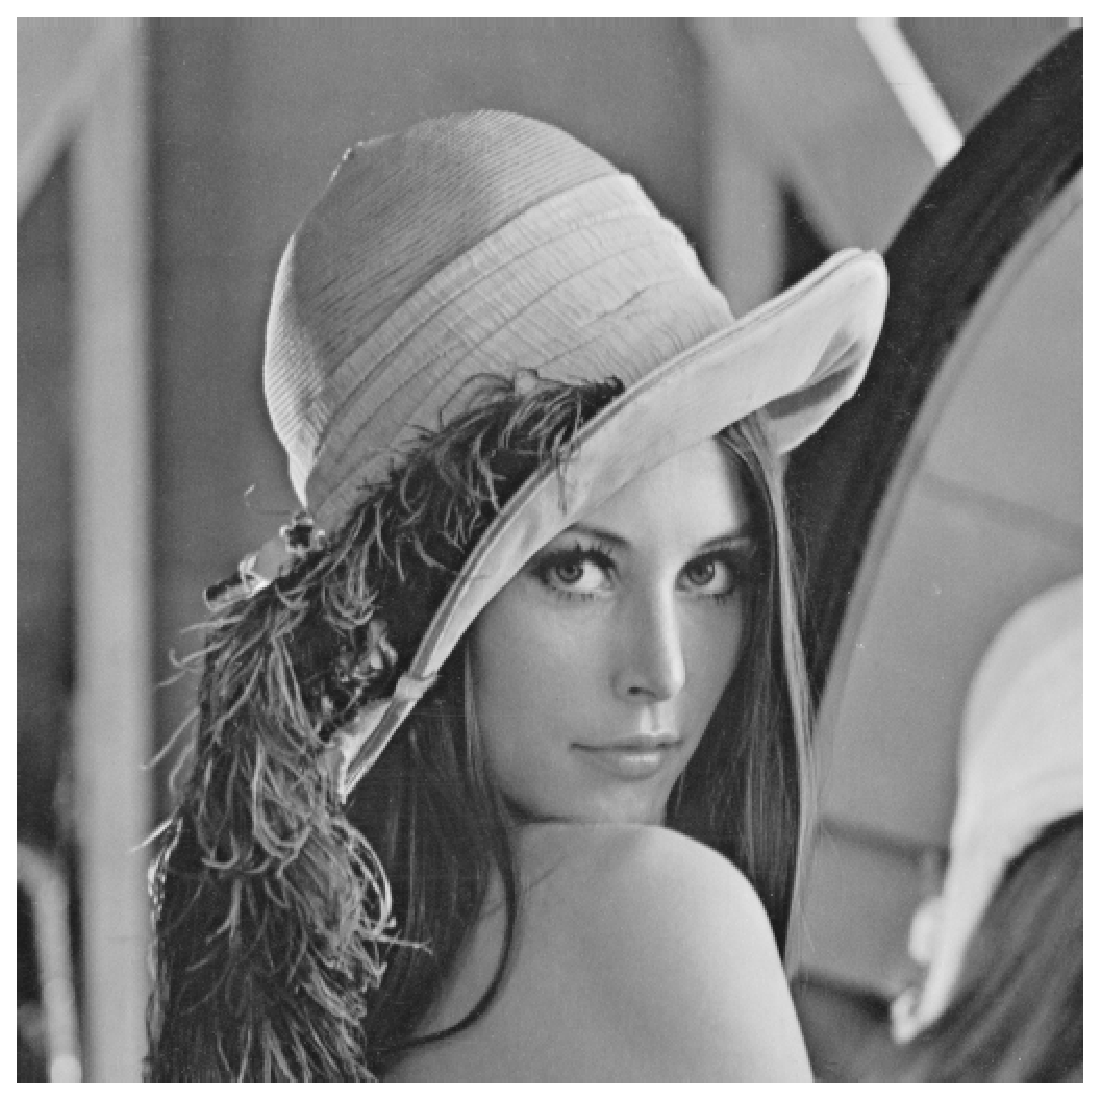
\includegraphics[width=0.45\linewidth]{lena} 
	\caption[Titre pour la liste des figures]{On pourra mettre ce qu'on veut sous la figure, le titre dans la table des figures demeurera court.}
	\label{fig:figureSeule}
\end{figure}

Le paquet \texttt{subfigure} vous permet d'avoir plusieurs images dans la même figure et des légendes différentes pour chacune. Vous pourrez référer à la figure entière ou à chaque sous-figure individuelle. Seul le titre principal de la figure se retrouvera dans la liste au début du document.

% \begin{figure}[t] 
% 	\centering
% 	\subfigure[Image du caméraman]{\label{subfig:camera}	
% 		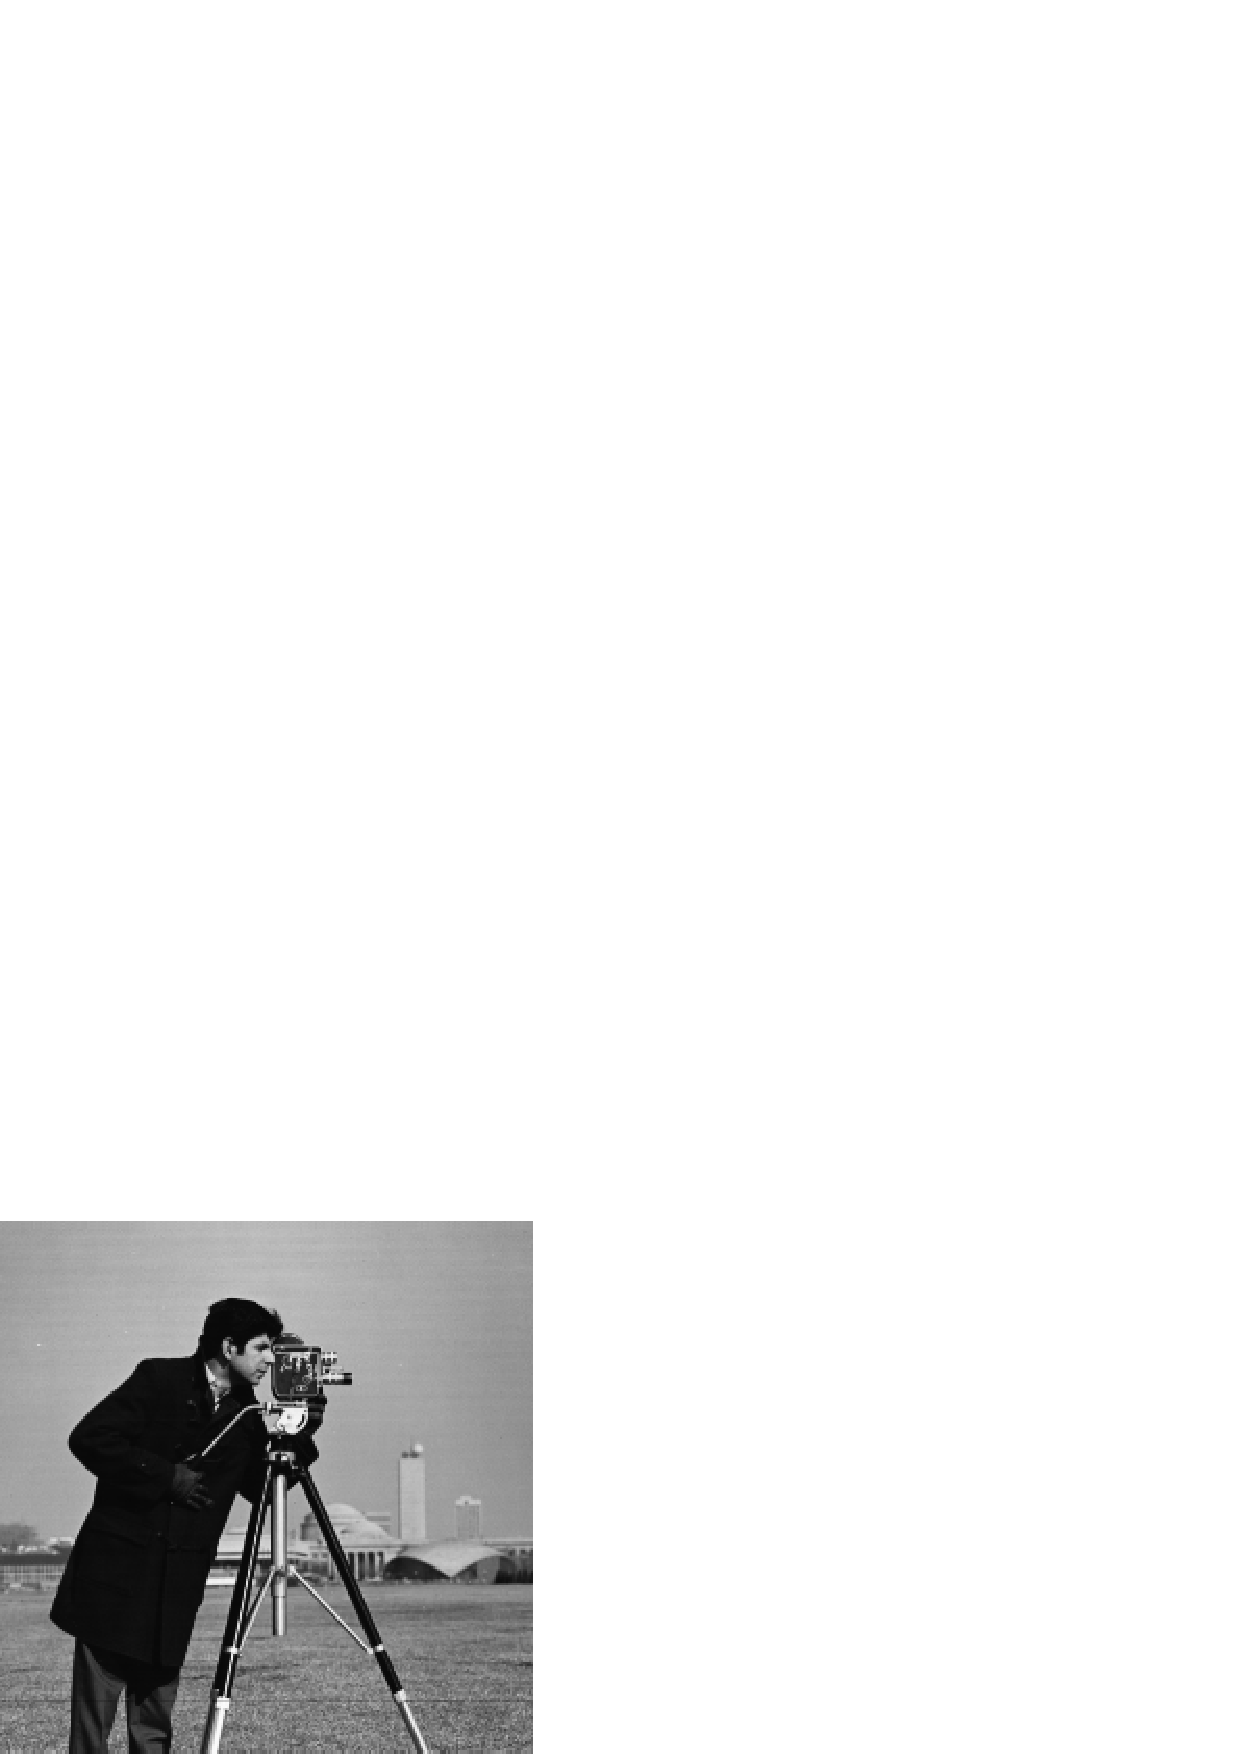
\includegraphics[width=0.25\linewidth]{camera.png}}
% 	\subfigure[Image de Lena]{\label{subfig:lena}
% 		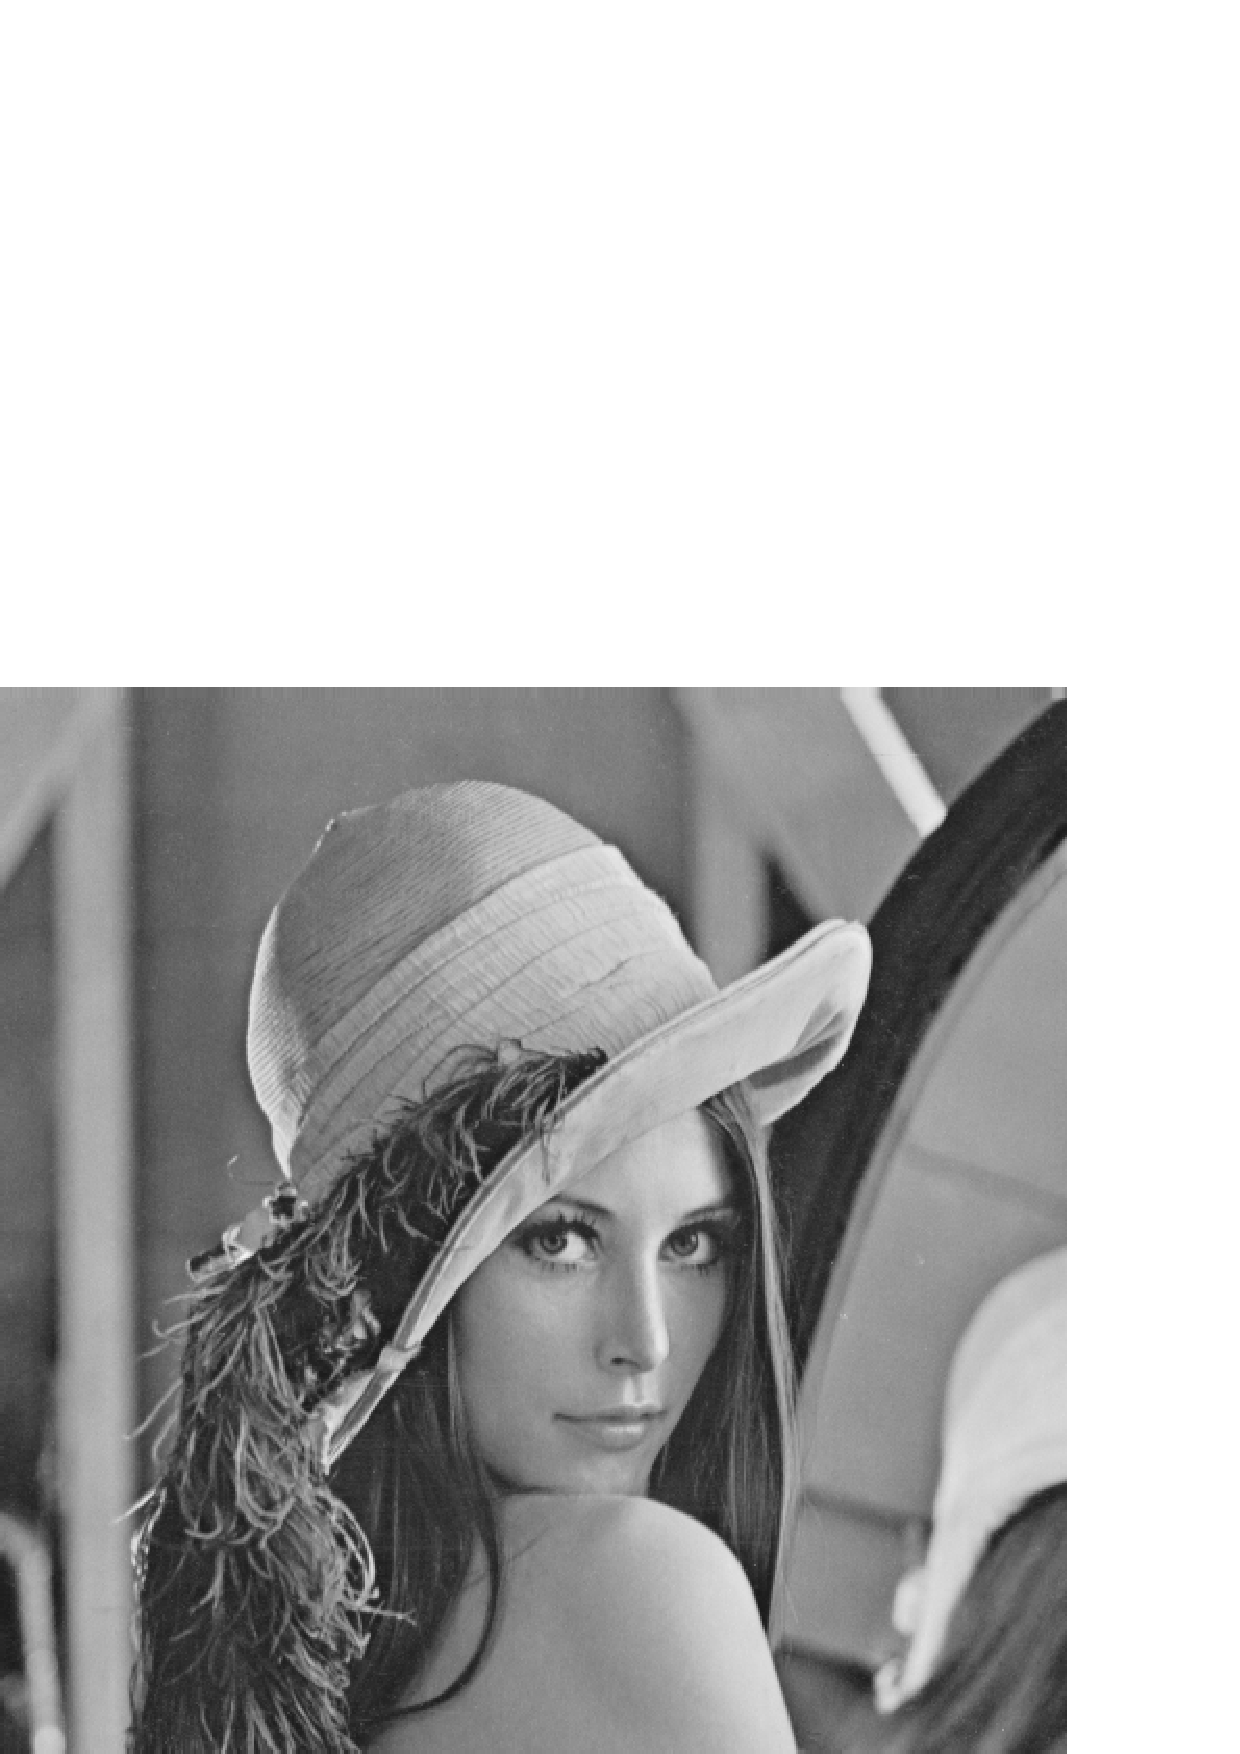
\includegraphics[width=0.25\linewidth]{lena.png}}
% 	\caption[Exemple d'inclusion de sous-figures]{Exemple d'inclusion de figures avec
% 		deux sous-figures pouvant avoir des légendes indépendantes. Elles peuvent être référencées de façon individuelles (voir \secref{refs}).} \label{fig:twoImages}
% \end{figure}

\clearpage

Des fois, latex accumule les éléments flottants avant de les placer dans le document et cela peut causer des problèmes. Il est bon de mettre la commande \verb|\clearpage| de temps en temps pour que les éléments flottants soient affichés dans les prochaines pages.

\section{Équations}
%%%%%%%%%%%%%%%%%%%%%%%%%%%%%%%%%%%%%%%%%%%%%%%%%%%%%%%%%%%%

Exemple d'une équation référencée dans le texte~:
\begin{equation}\label{eq:heatConserv}
	\nabla \cdot (\kappa \nabla u) = f.
\end{equation}

La suivante ne l'est pas alors on ne la numérote pas~:
\begin{equation*}
	\vec{v}(X,t)
	= \frac{dx}{dt} = \vec{v}(x,t).
\end{equation*}

\section{Tableaux}
%%%%%%%%%%%%%%%%%%%%%%%%%%%%%%%%%%%%%%%%%%%%%%%%%%%%%%%%%%%%

Le paquet \texttt{booktabs} vous permet de faire des tableaux plus agréables à l'oeil (voir \tabref{table1} et \url{https://www.ctan.org/pkg/booktabs} pour la documentation).

\begin{table}
	\centering
	\begin{tabular}{c c c}
		\toprule
		\textbf{Image}   & \textbf{Hello}   & \textbf{World}\\
		\hline
		\textbf{Ex1}  & $32$                  & 13.55 \\
		\textbf{Ex2}    & $5$                   & 48.20    \\
		\textbf{Ex3}    & $113$                 & 12.06    \\
		\bottomrule
	\end{tabular}
	\caption[Exemple d'un beau tableau]{Exemple d'un beau tableau avec un long
		titre.} \label{tab:table1}
\end{table}

\section{Légendes}
\label{sec:legendes}
%%%%%%%%%%%%%%%%%%%%%%%%%%%%%%%%%%%%%%%%%%%%%%%%%%%%%%%%%%%%


Utilisez l'option \texttt{Titre court} de \texttt{caption} pour éviter les noms trop longs dans les listes des pages préliminaires du document~:

\begin{verb}
	\caption[Titre court]{Titre long}
\end{verb}.

remarque faire la liste des préfixes à utiliser pour utiliser autoref et refstyle.

\section{Étiquettes}
\label{sec:etiq}
%%%%%%%%%%%%%%%%%%%%%%%%%%%%%%%%%%%%%%%%%%%%%%%%%%%%%%%%%%%%

Le paquet \texttt{refstyle} permet de faciliter la manipulation des étiquettes et surtout des références croisées (voir \secref{refs}). 

Afin de permettre une utilisation optimale des références croisées faciles, il est de requis de préfixer chaque étiquette du type d'élément à laquelle elle fait référence (\url{https://en.wikibooks.org/wiki/LaTeX/Labels_and_Cross-referencing#cite_note-:0-6}).

Voici les types qui sont définis et dont la version française est fournie pour utiliser \texttt{refstyle} :

\begin{itemize}
	\item[part:] partie
	\item[chap:] chapitre ou annexe
	\item[sec:]  section
	\item[subsec:] subsection
	\item[fig:] figure
	\item[subfig:] sous-figure
	\item[tab:] tableau
	\item[eq:] équation
	\item[lst:] recopie de code
	\item[itm:] item d'une liste
	\item[algo:] algorithme
	\item[fn:] note de bas de page
\end{itemize}

Voir aussi les différentes sections de cette annexe pour des exemples d'étiquettage vous permettant d'utiliser le paquet \texttt{refstyle} correctement.

\newpage

\section{Algorithmes}
%%%%%%%%%%%%%%%%%%%%%%%%%%%%%%%%%%%%%%%%%%%%%%%%%%%%%%%%%%%%

Voici un exemple d'algorithme entré dans l'environnement \texttt{algorithmic} dont les mots-clés seront en français si le document est en français. Vous pouvez adapter ou enlever la francisation dans le document \texttt{ajoutsFct.tex}.

\begin{algorithm}[H]
	\caption[Titre court]{Algorithme avec étiquette trop longue pour la liste du début}\label{algo:cap}
	\begin{algorithmic}
		\Require $n \geq 0$
		\Ensure $y = x^n$
		\State $y \gets 1$
		\State $X \gets x$
		\State $N \gets n$
		\While{$N \neq 0$}
		\If{$N$ is even}
		\State $X \gets X \times X$
		\State $N \gets \frac{N}{2}$  \Comment{commentaire}
		\ElsIf{$N$ is odd}
		\State $y \gets y \times X$
		\State $N \gets N - 1$
		\EndIf
		\EndWhile
	\end{algorithmic}
\end{algorithm}

\clearpage

\section{Codes sources}
%%%%%%%%%%%%%%%%%%%%%%%%%%%%%%%%%%%%%%%%%%%%%%%%%%%%%%%%%%%%

% https://en.wikibooks.org/wiki/LaTeX/Source_Code_Listings
%\lstset{language=C++}  % en dehors de l'environnement lstlisting
%\lstset{}

Il est possible de mettre des recopies de codes sources dans votre document. 

Voir \url{https://en.wikibooks.org/wiki/LaTeX/Source_Code_Listings} pour plus d'information sur le paquet \texttt{lstlisting} dont vous avez quelques exemples d'utilisation ici.

Préférez l'inclusion des codes assez courts (moins d'une page) dans des environnements flottants. Sinon, le code sera traité comme du texte concernant le placement, à privilégier pour du code plus long qu'une page. Cette dernière option devrait être utilisée avec parcimonie.

\begin{lstlisting}[
	language=Python, 
	caption={[Titre court du code] Ceci est un code en C++ écrit directement dans le fichier \texttt{.tex}},
	label=lst:tex,
	% autres options disponibles
]
import numpy as np

def incmatrix(genl1,genl2):
	m = len(genl1)
	n = len(genl2)
	M = None #to become the incidence matrix
	VT = np.zeros((n*m,1), int)  #dummy variable
	
	#compute the bitwise xor matrix
	M1 = bitxormatrix(genl1)
	M2 = np.triu(bitxormatrix(genl2),1) 
	
	for i in range(m-1):
		for j in range(i+1, m):
			[r,c] = np.where(M2 == M1[i,j])
			for k in range(len(r)):
				VT[(i)*n + r[k]] = 1;
				VT[(i)*n + c[k]] = 1;
				VT[(j)*n + r[k]] = 1;
				VT[(j)*n + c[k]] = 1;
	
				if M is None:
					M = np.copy(VT)
				else:
					M = np.concatenate((M, VT), 1)
				
				VT = np.zeros((n*m,1), int)
	
	return M
\end{lstlisting}

\begin{lstlisting}[
	float, 			% environnement flottant
	language=c++ ,
	caption=A floating example, 
	nolol,    % enlève l'entrée de la liste des codes sources.
]
Carte::Carte(unsigned int i_nDim) :
m_nDimension{i_nDim}
{
	// Creation du tableau des valeurs
	vector<unsigned int> vecColonne (i_nDim, 0);
	m_tab.assign(i_nDim, vecColonne);
	m_nNbCasesVides = m_nDimension * m_nDimension;
	unsigned int premierChiffre ;
	premierChiffre = genereChiffre(Direction(random::genereValeur(0, 3)));
	m_nMax = premierChiffre;
};
\end{lstlisting}

\lstinputlisting[
	float, 					% environnement flottant
	caption={Code en python inclus en partie à partir d'un fichier dans un float},
	label=lst:incl, 
	language=Python, 
	firstline=2, lastline=12, % première et dernière ligne à inclure
]{annexes/exempleCodePython.py}

\clearpage

\lstinputlisting[
	caption={Code en python inclus à partir d'un fichier mais pas dans un float},
	label=lst:nonfloat, 
	language=Python,
]{annexes/exempleCodePython.py}

\section{Références croisées}
\label{sec:refs}
%%%%%%%%%%%%%%%%%%%%%%%%%%%%%%%%%%%%%%%%%%%%%%%%%%%%%%%%%%%%

Vous pouvez toujours utiliser la façon régulière de faire vos références croisées, en utilisant simplement \verb@\ref{etiquette}@, \verb|\nameref{etiquette}| \\
ou \verb@\pageref{etiquette}@.

\begin{quote}
	Les chapitres \ref{chap:chapitre1} et \ref{chap:soumis}. Le nom du chapitre de conclusion est \nameref{chap:conclusion} et sa page est \pageref{chap:conclusion}. 
\end{quote}

Vous avez aussi deux façons alternatives: les références automatiques (\subsecref{autoref}) et l'utilisation de \texttt{refstyle} (\subsecref{refstyle}).

\subsection{Références automatiques}
\label{subsec:autoref}
%%%%%%%%%%%%%%%%%%%%%%%%%%%%%%%%%%%%%%%%%%%%%%%%%%%%%%%%%%%%

%\modeFrancais

Il est possible d'obtenir des liens plus lisibles (incluant le type d'objet dans le lien) avec \texttt{autoref}. La traduction du terme est automatique aussi.
Par exemple :

\begin{quote}
Le \autoref{chap:chapitre1} et le \autoref{chap:soumis}. La page du chapitre de conclusion est \autopageref{chap:conclusion}.

Pour les différents éléments, la commande choisit le meilleur terme : \autoref{chap:latex}, \autoref{eq:heatConserv}, \autoref{fig:figureSeule}, \autoref{lst:incl}, \autoref{sec:abbrev}, \autoref{subsec:autoref}, \autoref{tab:table1}, \autoref{algo:cap}.
\end{quote}

Ceci est à comparer à
\begin{quote}
	Le chapitre \ref{chap:chapitre1} et le chapitre \ref{chap:soumis}. La page du chapitre de conclusion est \pageref{chap:conclusion}.
	
	Pour les différents éléments, la commande ne choisit pas le meilleur terme, il faut l'ajouter explicitement : annexe \ref{chap:latex}, équa. \ref{eq:heatConserv}, Figure \ref{fig:figureSeule}, code \ref{lst:incl}, section \ref{sec:abbrev}, sous-section \ref{subsec:autoref}, tableau \ref{tab:table1}
\end{quote}

\subsubsection{Désavantages}

La commande \texttt{autoref} pose certains désavantages, elle n'offre pas un niveau de contrôle élevée : 

\begin{itemize}
	\item Il n'y a pas de contrôle sur la première lettre qui ne peut se mettre en majuscule.
	\item On ne peut pas mettre plusieurs étiquette dans la même commande.
\end{itemize}

Le paquet \texttt{refstyle} remédie à ces problèmes mais n'offre pas la possibilité d'inclure le nom de l'élément dans le lien sauf pour les chapitres et annexes.

\subsection{Utilisation de \texttt{refstyle}}
\label{subsec:refstyle}
%%%%%%%%%%%%%%%%%%%%%%%%%%%%%%%%%%%%%%%%%%%%%%%%%%%%%%%%%%%%

Pour bien utiliser \texttt{refstyle}, il faut étiqueter correctement les éléments en utilisant les préfixes par type (voir \secref{etiq}).
Par exemple la référence à l'équation étiquetée \texttt{eq:HeatConserv} indique que l'élément est une équation. Si on utilise \verb|\eqref{HeatConserv}| (notez le passage du préfixe de l'étiquette vers un préfixe équivalent de la commande de référence, sans les «:»), on inclue le type de l'élément dans la référence.

Pour les différents éléments, la commande choisit le terme à inclure dépendamment du préfixe de la commande.
\begin{quote}
	Le \chapref{chapitre1} et le \chapref{soumis}. 
	
	\chapref{latex}, \eqref{heatConserv}, \figref{figureSeule}, \lstref{incl}, \secref{abbrev}, \subsecref{autoref}, \tabref{table1}, \algoref{cap}
\end{quote}

Il est possible de mettre la première lettre en majuscule : \Eqref{heatConserv}.

Le pluriel ainsi que les mots de liens se font automatiquement en mettant plusieurs étiquettes du même type,  séparées par des virgules, dans la référence.

Dans la \figref{twoImages}, nous avons deux images, c'est-à-dire, les \subfigref{camera, lena}.

Le no. de page : \subfigpageref{camera}. 

Le nom de la section contenant un élément \nameref{algo:cap}.

Référence à la \secref{legendes}. Référence aux \subsecref{refstyle, three}.

Références aux \subsecref{autoref, refstyle, three} ou aux \lstrangeref{tex}{nonfloat} .

\subsection{Langue des références dans le texte}
\label{subsec:three}
%%%%%%%%%%%%%%%%%%%%%%%%%%%%%%%%%%%%%%%%%%%%%%%%%%%%%%%%%%%%

Il est possible de changer le mode de langue pour passer à l'anglais (utilisation de \verb|\modeAnglais|, \verb|\modeFrancais|, \verb|\modeDefaut|) autant avec \texttt{autoref} qu'avec \texttt{refstyle}.

On passe au mode anglais (\verb|\modeAnglais|).
\modeAnglais

\begin{quote}
	\texttt{autoref}:
	
	Le \autoref{chap:chapitre1} et l'\autoref{chap:latex}. La page du chapitre de conclusion est \autopageref{chap:conclusion}. Autres exemples : \autoref{eq:heatConserv}, \autoref{fig:figureSeule}, \autoref{lst:incl}, \autoref{sec:abbrev}, \autoref{subsec:autoref}, \autoref{tab:table1}.
	
	\texttt{refstyle}:
	
	Le \chapref{chapitre1} et le \chapref{latex}. Autres exemples : \eqref{heatConserv}, \figref{figureSeule}, \lstref{incl}, \secref{abbrev}, \subsecref{autoref}, \tabref{table1}, \algoref{cap}, \Eqref{heatConserv}, \subfigref{camera, lena}, \subfigpageref{camera}, \subsecref{autoref, refstyle, three}, \lstrangeref{tex}{nonfloat}.
\end{quote}

On revient au mode français (\verb|\modeFrancais|) .
\modeFrancais

\begin{quote}
		\texttt{autoref}:
	
	Le \autoref{chap:chapitre1} et l'\autoref{chap:latex}. La page du chapitre de conclusion est \autopageref{chap:conclusion}. Autres exemples : \autoref{eq:heatConserv}, \autoref{fig:figureSeule}, \autoref{lst:incl}, \autoref{sec:abbrev}, \autoref{subsec:autoref}, \autoref{tab:table1}.
	
	\texttt{refstyle}:
	
	Le \chapref{chapitre1} et l'\chapref{latex}. Autres exemples : \eqref{heatConserv}, \figref{figureSeule}, \lstref{incl}, \secref{abbrev}, \subsecref{autoref}, \tabref{table1}, \algoref{cap}, \Eqref{heatConserv}, \subfigref{camera, lena}, \subfigpageref{camera}, \subsecref{autoref, refstyle, three}, \lstrangeref{tex}{nonfloat}.
\end{quote}

\modeDefaut

\section{Abréviations}
\label{sec:abbrev}
%%%%%%%%%%%%%%%%%%%%%%%%%%%%%%%%%%%%%%%%%%%%%%%%%%%%%%%%%%%%

Si vous avez des définitions d'abréviations utilisant\\
\begin{verb}
	\newabbreviation{etiquette}{ABR}{Expression à remplacer},
\end{verb}\\
il devient facile d'insérer rapidement celles-ci dans le texte avec seulement l'étiquette en utilisant \verb|\gls{etiquette}|. À la première utilisation, elle sera automatiquement étendue avec l'abbréviation entre parenthèses.
\begin{quote}
	\gls{etiquette}, vs \gls{etiquette} vs \glsentryfull{etiquette}.
\end{quote}

Voir \url{https://en.wikibooks.org/wiki/LaTeX/Glossary} pour plus de détails.
 % fichier SpecLatex.tex
	
	%%=========================== ANNEXE PRÉCISIONS BIBTEX ============================
	
%	\modeDefaut
%	% !TeX spellcheck = fr_FR

\chapter{Comment utiliser bibtex}
\label{app:bibtex}

Les notices de la bibliographie doivent \^etre mises dans un document \texttt{.bib}. La bibliographie de ce gabarit est située dans le fichier \texttt{bibliographie.bib} (précisé dans le document principal). Vous y trouverez une panoplie d'exemples de notices de toutes sortes. C'est \LaTeX~avec bibtex qui s'occupe de classer et d'int\'egrer les bons liens dans votre document, ainsi que de g\'en\'erer la bibliographie correctement.

Il y a plusieurs types de documents pouvant \^etre utilis\'es:
\begin{description}
	\item[book] livre (exemples~\cite{Abr.96-BBook,Hoa.85-CSP, Jac.83-JSD,Mil.89-CCS});
	\item[manual] manuel d'utilisation, sensiblement \'equivalent \`a un livre \cite{STE.97-Manuel-B};
	\item[inbook] chapitre d'un livre(exemple ~\cite{Ch.96-Programmer-avec-Scheme, kevorkian90});
	\item[article] article de recherche classique publi\'e dans un journal (et non une conf\'erence) (exemples \cite{Bo.84-VVS,FFL.05-SOSYM,FSd.03-eb3});
	\item[proceedings] les actes d'une conf\'erence (exemples \cite{ArGnMa.03-FME, LeWe.09-IFM});
	\item[inproceedings] parution dans un acte de conf\'erence (exemples \cite{Matra.99-Meteor,FF.07-ICFEM,Pn.79-The-Temporal-Semantics-of-Concurrent-Programs}) \'eventuellement avec une r\'ef\'erence crois\'ee  (\texttt{crossref}) (exemple \cite{LeBu.03-ProB});
	\item[conference] identique au pr\'ec\'edent;
	\item[phdthesis] th\`ese de doctorat (\cite{FRA.06-thesis});
	\item[masterthesis] m\'emoire de ma\^itrise (\cite{Ri.01-EB3});
	\item[techreport] rapport de recherche paru dans une institution (universitaire ou autre) et disponible publiquement (\cite{FRA.05-TR9});
	\item[incollection] article d'une collection d'articles parus ailleurs (\cite{BB.89-LOTOS, CitekeyIncollection});
	\item[booklet] livret ou un document comme une th\`ese d'habilitation \`a diriger la recherche ou un manuel utilisateur (\cite{La.02-CDBD,STE.97-Manuel-B});
	\item[unpublished] document non publi\'es, par exemple pour cause de confidentialit\'e (\cite{deschenes98, BuDo.99-guide-B});
	\item[misc] n'importe quel autre document, utile pour un site Internet ou un document publié sur un site personnel (\cite{INRIA.cadp, Gi.08-Logic-Vs.-Intelligence}). On évitera ce genre de référence dans la bibliographie puisqu'elle est hautement volatile.
\end{description}

Les références des articles \cite{FRA.05-TR9, FF.07-ICFEM} illustrent pourquoi on ne doit, en général pas mettre de lien URL vers un article puisque l'éditeur des résumés a réorganisé son site et l'adresse n'est plus valide. L'usage d'un identifiant numérique d'objet (DOI, \textit{Digital object identifier}) si disponible est plus pertinent : \cite{FF.07-ICFEM, FFL.05-SOSYM} pour trouver l'article sur Internet \cite{Uqam.presGuide.18} \footnote{Veuillez consulter le site \\
\url{http://bib-it.sourceforge.net/help/fieldsAndEntryTypes.php} pour plus de détails}.

Les commandes de référence standards de base sont :
\begin{itemize}
	\item Référence unique : \cite{Abr.96-BBook};
	\item Références multiples : \cite{deriche95, tschumperle02, weickert97};
	\item Références par le nom des personnes autrices (avec lien) : \citeauthor{deriche95}.
\end{itemize}
La dernière option devrait être utilisée lorsque le document a déjà été référé avec son numéro dans du texte qui précède d'assez près.

\section{Natbib}

Avec le paquet \texttt{natbib} inclus dans la classe (options crochets et numéros)

Références uniques :
\begin{itemize} 
	\item Numéro seul : \citep{deriche95};
	\item Nom des personnes autrices et numéro de la notice : \citet{deriche95};
	\item Nom des personnes autrices sans numéro (avec lien) : \citeauthor{deriche95};
	\item Année de la publication (avec lien) : \citeyear{deriche95};
	\item Précision de l'endroit dans le document : \citep[chap. 2]{deriche95};
	\item Ajout d'une note au préalable : \citep[par exemple][]{Essen2012};
	\item Précision de l'endroit et note préalable : \citep[p.ex.][p. 32]{Essen2012}.
\end{itemize}


Références multiples :
\begin{itemize} 
	\item Numéros seuls : \citep{auclair02a, tschumperle02, weickert97};
	\item Nom des personnes autrices et numéros des notices : \citet{auclair02a, tschumperle02, weickert97};
	\item Nom des personnes autrices sans numéro : \citeauthor{auclair02a, tschumperle02, weickert97};
	\item Années de publication : \citeyear{auclair02a, tschumperle02, weickert97}.
\end{itemize}

\section{Noms des auteurs et autrices}

Lorsque la liste des auteurs et autrices contient beaucoup de noms, les deux styles de bibliographies fournis (\texttt{UdeSDIfr.bst} et \texttt{UdeSDIeng.bst}) remplacent les derniers auteurs par \textit{et al.}. Par exemple la notice dans le fichier .bib se lit comme suit:
\begin{lstlisting}[nolol,numbers=none,frame=]
@article{Essen2012,
	author = {Essen, D.C. and Ugurbil, K and Auerbach, Edward and Barch, Deanna and Behrens, T.E.J. and Bucholz, Richard and Chang, A and Chen, Liyong and Corbetta, Maurizio and Curtiss, Sandra and Della Penna, Stefania and Feinberg, David and Glasser, Matthew and Harel, Noam and Heath, A.C. and Larson-Prior, Linda and Marcus, Daniel and Michalareas, Georgios and Moeller, Steen and Yacoub, Essa},
	year = {2012},
	month = {02},
	pages = {2222-31},
	title = {The Human Connectome Project: A data acquisition perspective},
	volume = {62},
	journal = {NeuroImage},
	doi = {10.1016/j.neuroimage.2012.02.018}}
\end{lstlisting}

Notez que la notice visible dans la bibliographie ne contient que six des noms des auteurs et que les prénoms ont été remplacés par l'initiale du premier prénom :
% TODO: \usepackage{graphicx} required
\begin{center}
	\includegraphics[width=\linewidth]{"Notice"}
\end{center}

Exemples de citations dans le texte :

\begin{itemize}
	\item Noms des six premiers auteurs et numéro : \citet*{Essen2012}
	\item Nom du premier auteur sans numéro (avec lien) : \citeauthor{Essen2012}
	\item Noms des six premiers auteurs sans numéro (avec lien) : \citeauthor*{Essen2012}	
\end{itemize}

Il est aussi possible d'ajouter dans la notice \texttt{and others} pour remplacer tous les derniers auteurs ou autrices par un terme générique.

\begin{lstlisting}[nolol,numbers=none,frame=]
@book{kevorkian90,
	author = {J. Kevorkian and others},
	title = {{Partial Differential Equations : Analytical Solution Techniques}},
	...
\end{lstlisting}

Notez que le terme \texttt{others} a été remplacé dans la notice visible comme suit.
\begin{center}
	\includegraphics[width=\linewidth]{"NoticeEtal"}
\end{center}

 % fichier annexe-Bibtex.tex
	
% La commande suivante fait en sorte que toutes les entrées d'abréviations définies dans le fichier prelim sont incluses dans la liste
% si ce comportement n'est pas souhaité, mettre en commentaires.
\glsaddallunused

\end{document}

